\documentclass[12pt,a4paper]{article}

\usepackage{fontspec}
\setmainfont{Times New Roman}

\usepackage[margin=2.5cm]{geometry}
\usepackage{amsmath}
\usepackage{graphicx}
\usepackage{booktabs}
\usepackage{caption}
\usepackage{longtable}
\usepackage{hyperref}
\usepackage{xurl}
\usepackage{xcolor}
\usepackage{float}

\renewcommand{\figurename}{Hình}
\renewcommand{\tablename}{Bảng}
\renewcommand{\contentsname}{Mục lục}

\hypersetup{
  colorlinks=true,
  linkcolor=black,
  urlcolor=blue,
  citecolor=black,
}

\graphicspath{{../A1/figures/}}

\title{\textbf{Báo cáo A1.2: So sánh CNN và Transformer trên Food-101}\\[0.3em]
\large Học sâu và ứng dụng trong thị giác máy tính\\
Mã môn học: CO5085, Học kỳ 261 (2026--2027)}

\author{
Nguyễn Xuân Trường (2570526) \\
Trần Lê Hoàng Long (2570443)
}
\date{Cập nhật lần cuối: 09/11/2026}

\begin{document}

\maketitle

\vspace{1cm}
\begin{center}
\begin{tabular}{ll}
\textbf{Giảng viên hướng dẫn:} & Lê Thành Sách, Nguyễn Quốc Minh \\
\textbf{Repository:} & \url{https://github.com/truong1501/SDH_HK261_CO5085} \\
\textbf{Protocol:} & \texttt{reports/A1.1\_Dataset-Protocol.pdf} \\
\end{tabular}
\end{center}

\vspace{0.5cm}
\begin{center}
\begin{minipage}{0.85\linewidth}
\textbf{Tóm tắt.} Nhóm huấn luyện ResNet-50 (CNN) và DeiT-Small (ViT thuần) trên
Food-101 theo bốn chế độ: from-scratch, freeze toàn bộ backbone, freeze một phần
và full finetune, đúng protocol đã nộp ở A1.1. Tổng cộng 24 lần huấn luyện (20 lần
cho bảng chính, 4 lần dò learning rate), khoảng 8,4 giờ A100. Với pretrained
ImageNet-1k, DeiT-S tốt hơn ResNet-50 ở cả ba chế độ (full finetune: 88,62\% so với
85,65\% top-1). Khi train từ đầu thì ngược lại: ResNet-50 đạt 82,48\%, DeiT-S chỉ
67,13\%. Pretrain giúp DeiT-S thêm 21,5 điểm nhưng chỉ giúp ResNet-50 thêm 3,2
điểm. Freeze một phần của DeiT-S giữ được gần hết accuracy của full finetune
(87,25\%) với một nửa số tham số trainable.
\end{minipage}
\end{center}

\clearpage
\tableofcontents
\clearpage

% =====================================================================
\section{Mục tiêu và câu hỏi nghiên cứu}

Đề bài A1 yêu cầu so sánh một mô hình CNN và một mô hình Transformer trên cùng một
tập dữ liệu ảnh, ở các mức tận dụng trọng số pretrained khác nhau. Ở A1.1, nhóm đã
chốt tập dữ liệu (Food-101), cặp mô hình (ResNet-50 và DeiT-Small), bốn chế độ
huấn luyện và toàn bộ siêu tham số trước khi chạy. Báo cáo này trình bày kết quả
của phần A1.2 và đối chiếu với protocol đó.

Protocol đặt ra ba câu hỏi:
\begin{enumerate}
\item Pretrain giúp CNN và ViT đến mức nào trên một tập khoảng 75 nghìn ảnh train?
\item Mức freeze nào cân bằng tốt nhất giữa accuracy và chi phí (thời gian, tham số
trainable, bộ nhớ)?
\item (Mở rộng) Transformer phân cấp như Swin có bớt phụ thuộc vào pretrain hơn ViT
thuần không?
\end{enumerate}

Câu 1 và 2 thuộc phần bắt buộc và được trả lời đầy đủ ở mục~\ref{sec:analysis}.
Câu 3 cần cặp mở rộng ConvNeXt-T/Swin-T (X1--X8). Nhóm chưa chạy cặp này nên
không đưa ra kết luận cho câu 3 (mục~\ref{sec:limits}).

\paragraph{Vì sao chọn ResNet-50 và DeiT-S.} ResNet-50 [2] và DeiT-S [3] có cỡ gần nhau (23,7M và
21,7M tham số sau khi thay head 101 lớp, khoảng 4 GFLOPs mỗi ảnh $224\times224$) và
cùng dùng trọng số ImageNet-1k từ \texttt{timm}, nên chênh lệch kết quả chủ yếu đến
từ kiến trúc. ResNet-50 mang hai thiên kiến quy nạp (inductive bias) của
convolution: tính cục bộ (mỗi kernel chỉ nhìn một vùng nhỏ) và chia sẻ trọng số khi
trượt trên toàn ảnh. Theo cách của ViT [4], DeiT-S cắt ảnh thành $14\times14$ patch kích thước $16\times16$ và
cho self-attention nhìn toàn bộ ảnh ngay từ block đầu tiên. Cách này linh hoạt hơn,
nhưng mô hình phải tự học các quy luật không gian từ dữ liệu. Vì vậy trước khi chạy,
nhóm kỳ vọng DeiT-S phụ thuộc vào pretrain nhiều hơn ResNet-50.

% =====================================================================
\section{Dữ liệu}

\subsection{Food-101 và cách chia}

Food-101 [1] gồm 101 món ăn, mỗi lớp 750 ảnh train và 250 ảnh test chính thức. Ảnh
test đã được kiểm tra thủ công. Ảnh train được tác giả cố ý giữ nhiễu: một số ảnh
màu gắt, một số ảnh sai nhãn. Nhóm giữ nguyên tập test và tách 10\% ảnh train làm
validation theo kiểu phân tầng (stratified), seed 42. Chỉ số ảnh được lưu trong
\texttt{A1/splits/} và dùng chung cho mọi run.

\begin{table}[H]
\centering
\caption{Split dùng cho mọi run}
\begin{tabular}{lcccp{5cm}}
\toprule
Split & Nguồn & Ảnh/lớp & Tổng & Dùng để \\
\midrule
Train & 90\% train chính thức & 675 & 68.175 & Huấn luyện \\
Validation & 10\% train chính thức & 75 & 7.575 & Chọn checkpoint, chọn LR \\
Test & Test chính thức & 250 & 25.250 & Đánh giá một lần trên checkpoint đã chọn \\
\bottomrule
\end{tabular}
\end{table}

Nhóm không dùng subset: toàn bộ 68.175 ảnh train được dùng cho mọi run.

\subsection{Khám phá dữ liệu}

Hình~\ref{fig:eda-sizes} cho thấy phần lớn ảnh có cạnh dài đúng 512 px (tác giả đã
thu nhỏ ảnh gốc về mức này), cạnh còn lại thường là 384 hoặc 512 px. Kích thước
không đồng đều nên mọi mô hình đều đưa ảnh về $224\times224$: lúc train dùng
RandomResizedCrop, lúc đánh giá dùng Resize 256 rồi CenterCrop 224.

\begin{figure}[H]
\centering
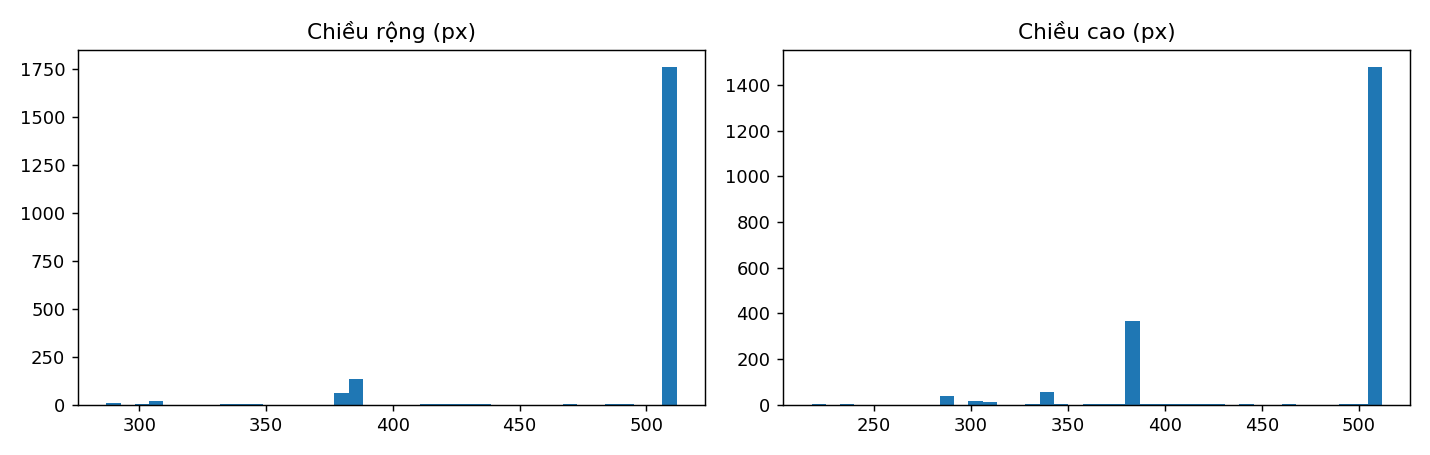
\includegraphics[width=\linewidth]{eda_sizes.png}
\caption{Phân bố chiều rộng và chiều cao của 2.000 ảnh train lấy ngẫu nhiên}
\label{fig:eda-sizes}
\end{figure}

\begin{figure}[H]
\centering
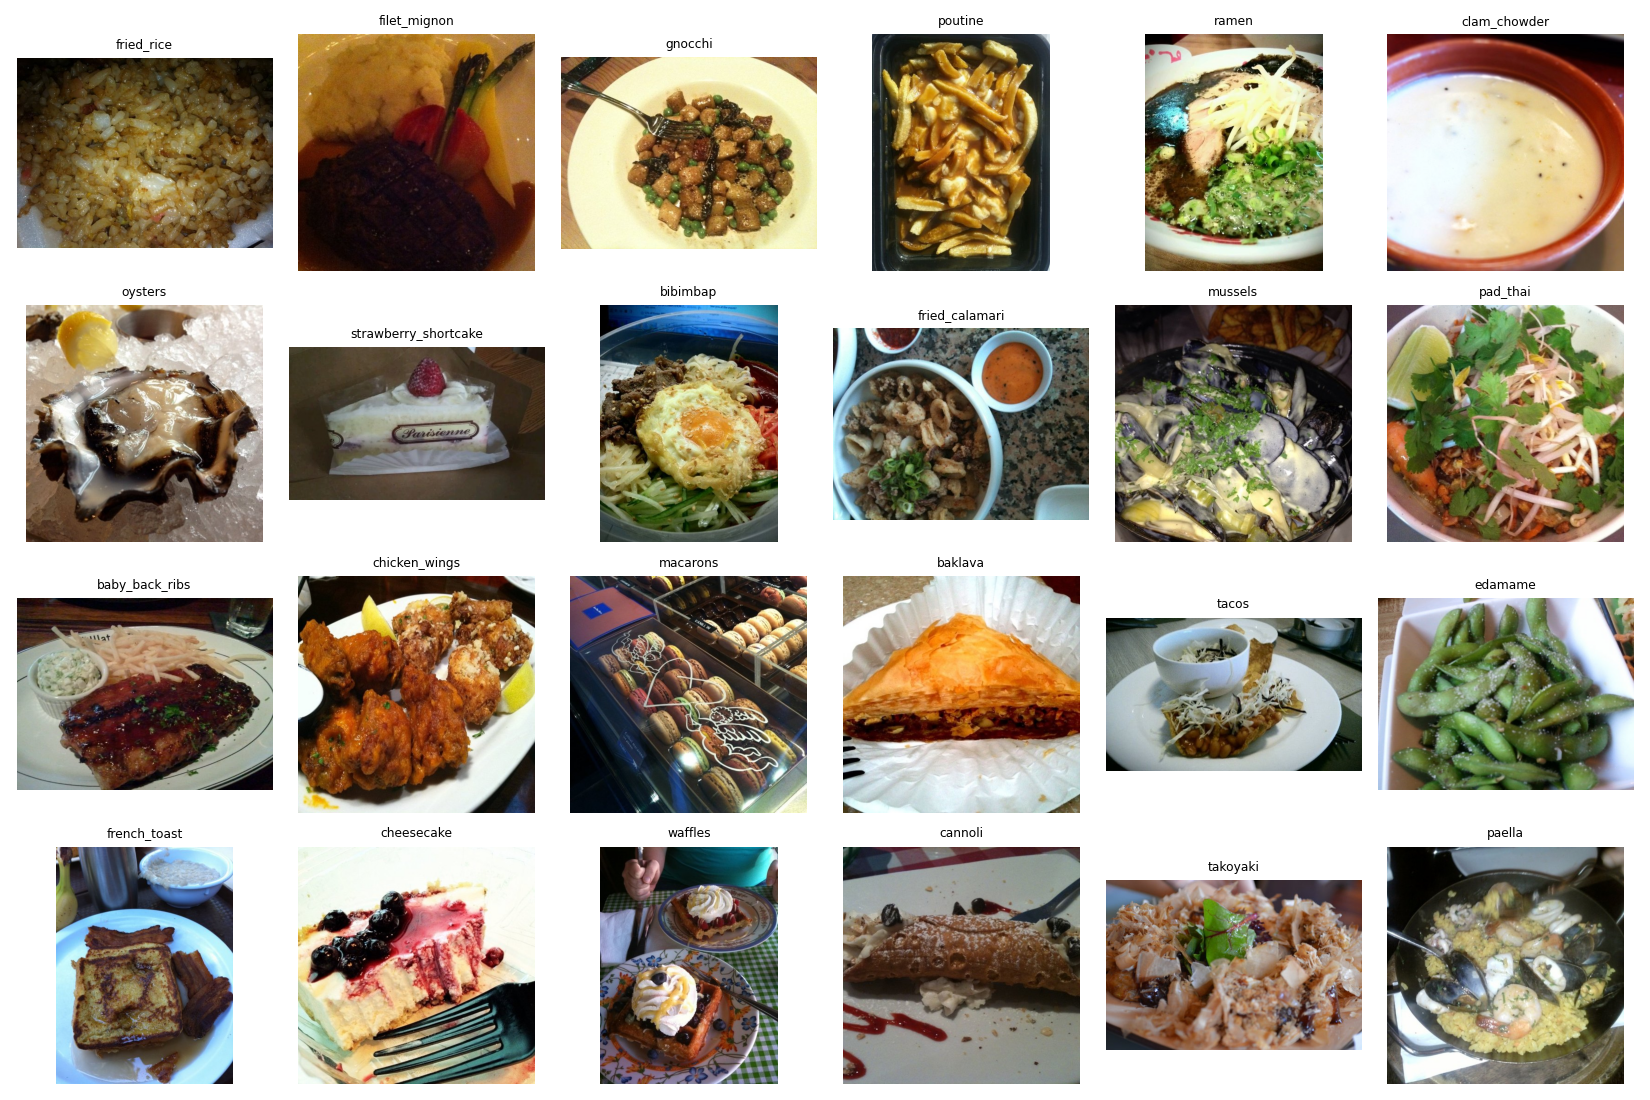
\includegraphics[width=\linewidth]{eda_samples.png}
\caption{Một ảnh train của 24 lớp chọn ngẫu nhiên. Nhiều món có màu sắc và cách bày
gần nhau; ánh sáng và góc chụp thay đổi nhiều vì ảnh do người dùng tự chụp}
\label{fig:eda-samples}
\end{figure}

Hai điểm từ bước này ảnh hưởng tới phần phân tích sau. Thứ nhất, ảnh có nền phức
tạp, thường có nhiều món trên cùng một bàn. Thứ hai, nhiều lớp chỉ khác nhau ở chi
tiết nhỏ hoặc cách chế biến (steak, filet mignon, prime rib, pork chop). Mục~\ref{sec:errors}
kiểm tra lại hai nhận xét này trên các ảnh mô hình đoán sai.

% =====================================================================
\section{Thiết lập thí nghiệm}

\subsection{Bốn chế độ huấn luyện}

\begin{table}[H]
\centering
\caption{Ma trận thí nghiệm. Số tham số trainable được đếm bằng code
(\texttt{p.requires\_grad}), đã gồm head 101 lớp}
\label{tab:matrix}
\small
\begin{tabular}{llllrc}
\toprule
ID & Mô hình & Khởi tạo & Phần được train & Trainable & Seed \\
\midrule
R1 & ResNet-50 & Ngẫu nhiên & Toàn bộ & 23,71M & 42 \\
R2 & ResNet-50 & Pretrained & Chỉ head & 0,21M & 42, 43, 44 \\
R3 & ResNet-50 & Pretrained & layer4 + head & 15,17M & 42, 43, 44 \\
R4 & ResNet-50 & Pretrained & Toàn bộ & 23,71M & 42, 43, 44 \\
\midrule
R5 & DeiT-S & Ngẫu nhiên & Toàn bộ & 21,70M & 42 \\
R6 & DeiT-S & Pretrained & Chỉ head & 0,04M & 42, 43, 44 \\
R7 & DeiT-S & Pretrained & Block 6--11 + norm cuối + head & 10,69M & 42, 43, 44 \\
R8 & DeiT-S & Pretrained & Toàn bộ & 21,70M & 42, 43, 44 \\
\bottomrule
\end{tabular}
\end{table}

``Freeze một phần'' được định nghĩa theo tỉ lệ tham số chứ không theo số stage:
khoảng 50--60\% tham số backbone được train. Với ResNet-50, nếu chỉ đóng băng hai
stage đầu thì chưa khóa được 10\% tham số, gần như không khác full finetune; vì vậy
nhóm đóng băng stem và layer1--layer3, chỉ train layer4. Với DeiT-S, nhóm đóng băng
patch embedding, position embedding, CLS token và block 0--5. Các lớp BatchNorm thuộc
phần bị đóng băng của ResNet-50 được giữ ở chế độ \texttt{eval()}, để mean/variance
học từ ImageNet không bị thống kê của từng batch Food-101 ghi đè. DeiT dùng
LayerNorm nên không gặp vấn đề này.

Ở chế độ freeze toàn bộ, backbone không đổi trong suốt quá trình train. Vì vậy nhóm
trích feature của mọi ảnh đúng một lần (khoảng 90 giây), lưu lại, rồi chỉ train lớp
tuyến tính trên feature đó; mỗi epoch chỉ còn khoảng nửa giây. Ba seed dùng chung
một bộ feature. Đổi lại, feature của ảnh train được trích bằng CenterCrop nên chế
độ này không có augmentation ngẫu nhiên. Đây là điểm khác với bảng augmentation của
protocol (vốn ghi RandomResizedCrop và HorizontalFlip), nhưng đã được nêu trong phần
``Freeze toàn bộ backbone'' ở mục 9 của protocol.

\subsection{Augmentation và siêu tham số}

Mức augmentation tăng theo số tham số được train. Trong cùng một chế độ, hai mô hình
dùng chung một pipeline.

\begin{table}[H]
\centering
\caption{Augmentation khi train. Khi đánh giá: Resize 256, CenterCrop 224, chuẩn hóa
ImageNet, không dùng test-time augmentation}
\begin{tabular}{p{4.3cm}p{10.7cm}}
\toprule
Chế độ & Augmentation \\
\midrule
Freeze toàn bộ & Feature trích từ CenterCrop 224 (không augmentation) \\
Freeze một phần, full finetune & RandomResizedCrop, HorizontalFlip, RandAugment (n=2, m=9),
RandomErasing (p=0,25) \\
From-scratch & Như trên + Mixup ($\alpha$=0,8) hoặc CutMix ($\alpha$=1,0) mỗi batch,
label smoothing 0,1 \\
\bottomrule
\end{tabular}
\end{table}

Augmentation mạnh cho from-scratch theo công thức của DeiT [3]: ViT thuần không có
inductive bias không gian nên rất dễ overfit trên 68 nghìn ảnh. ResNet-50 dùng đúng
công thức đó để khác biệt chỉ còn đến từ kiến trúc.

\begin{table}[H]
\centering
\caption{Siêu tham số. Mọi run dùng AdamW, warmup rồi cosine, batch 256, bf16}
\label{tab:hparams}
\begin{tabular}{lcccccc}
\toprule
Chế độ & Epoch & LR backbone & LR head & Warmup & Weight decay & Drop path \\
\midrule
From-scratch & 100 & 5e-4 & 5e-4 & 5 & 0,05 & 0,1 \\
Freeze toàn bộ & 30 & --- & 1e-3 & 0 & 0 & --- \\
Freeze một phần & 15 & theo dò LR & 1e-3 & 2 & 0,05 & 0,1 \\
Full finetune & 15 & theo dò LR & 1e-3 & 2 & 0,05 & 0,1 \\
\bottomrule
\end{tabular}
\end{table}

Head mới khởi tạo ngẫu nhiên nên dùng LR lớn hơn backbone: phần pretrained chỉ cần
điều chỉnh nhẹ, còn head phải học từ đầu. Checkpoint được chọn theo epoch có
validation top-1 cao nhất, và test chỉ được đánh giá một lần trên checkpoint đó.
Vòng lặp huấn luyện do nhóm tự viết bằng PyTorch, không dùng \texttt{Trainer.fit()}.

\subsection{Dò learning rate backbone}
\label{sec:lr}

Protocol không cố định LR backbone. Thay vào đó, với full finetune seed 42, nhóm thử
ba giá trị \{5e-5, 1e-4, 3e-4\}, chọn giá trị có validation top-1 cao nhất cho từng
mô hình, rồi dùng giá trị đó cho freeze một phần. Lý do: nếu hai mô hình dùng chung
một LR thì kết quả có thể nghiêng về mô hình hợp với LR đó hơn. Hai mô hình được dò
với cùng ngân sách (ba run mỗi mô hình) nên vẫn công bằng. Nhóm dùng luôn LR đã chọn
cho seed 43 và 44 của full finetune, để mean $\pm$ std được đo trên cùng một cấu hình.

\begin{table}[H]
\centering
\caption{Validation top-1 (\%) theo LR backbone, full finetune seed 42. Test không
tham gia vào việc chọn}
\label{tab:lr}
\begin{tabular}{lcccc}
\toprule
Mô hình & 5e-5 & 1e-4 & 3e-4 & LR được chọn \\
\midrule
ResNet-50 & 75,12 & 77,91 & \textbf{81,35} & 3e-4 \\
DeiT-S & 83,51 & \textbf{84,63} & 84,58 & 1e-4 \\
\bottomrule
\end{tabular}
\end{table}

\begin{figure}[H]
\centering
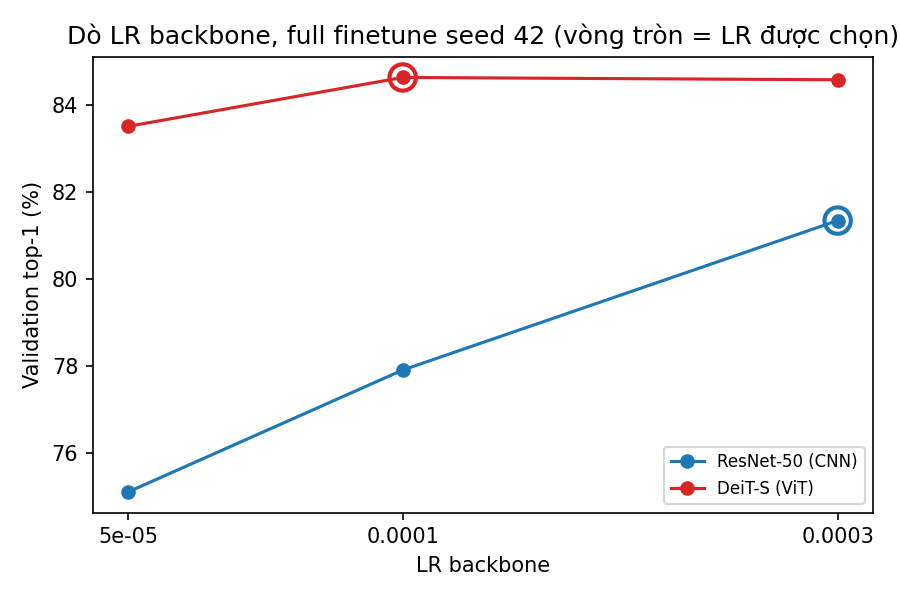
\includegraphics[width=0.75\linewidth]{lr_sweep.png}
\caption{Validation top-1 theo LR backbone (full finetune, seed 42)}
\label{fig:lr}
\end{figure}

Hai mô hình phản ứng rất khác với LR. ResNet-50 tăng đều khi LR tăng: từ 1e-4 lên 3e-4
được thêm 3,4 điểm validation. DeiT-S gần như phẳng giữa 1e-4 và 3e-4 (chênh 0,05
điểm). Nếu giữ nguyên LR mặc định 1e-4 của protocol, ResNet-50 sẽ bị đánh giá thấp
hơn thực tế khoảng 3,5 điểm top-1 trên test (82,17\% so với 85,66\% ở seed 42), và
khoảng cách CNN--ViT ở full finetune sẽ bị phóng đại hơn gấp đôi (6,4 thay vì 3,0 điểm). Đây là ví dụ cụ thể
cho thấy bước dò LR trong protocol là cần thiết. Một cách giải thích hợp lý là trọng
số \texttt{resnet50.a1\_in1k} được huấn luyện theo công thức A1 của timm với LR lớn [5], và mạng có BatchNorm nên
chịu được bước cập nhật lớn hơn. 3e-4 lại nằm ở biên lưới dò, nên LR tối ưu của
ResNet-50 có thể còn cao hơn (mục~\ref{sec:limits}).

\subsection{Phần cứng và cách chạy}

Mọi run chạy trên Google Colab với GPU A100, mixed precision bf16, PyTorch 2.14.1,
torchvision 0.29.1, timm 1.0.31. Toàn bộ R2 và R6, cùng R8 seed 42 và R4 seed 42
với LR 1e-4, chạy trên A100 80GB; các run còn lại chạy trên A100 40GB. Hai loại này có cùng
nhân tính toán, và thời gian mỗi epoch đo được gần như trùng nhau (Bảng~\ref{tab:all}).

Ảnh được copy từ Drive về ổ cục bộ của Colab ở đầu mỗi phiên, không đọc trực tiếp từ
Drive. Checkpoint được ghi lên Drive sau mỗi epoch (ghi ra file tạm rồi đổi tên để
không bao giờ còn lại file hỏng), nên khi Colab ngắt phiên, run tiếp tục từ epoch đã
lưu. Thứ tự chạy do \texttt{src/plan.py} quyết định: chạy seed 42 của đủ 8 run trước,
dò LR ở giữa vì R3/R7 cần kết quả dò, sau cùng mới đến seed 43 và 44.

% =====================================================================
\section{Kết quả}

\subsection{Bảng tổng hợp}

\begin{table}[H]
\centering
\caption{Kết quả trên test (\%). Run pretrained: mean $\pm$ std (độ lệch chuẩn mẫu)
qua 3 seed; from-scratch: 1 seed. Thời gian là tổng thời gian train một seed, freeze
toàn bộ đã gồm bước trích feature. VRAM là bộ nhớ GPU đỉnh khi train}
\label{tab:main}
\resizebox{\linewidth}{!}{%
\begin{tabular}{llcccccc}
\toprule
Run & Chế độ & LR bb. & Top-1 & Top-5 & Macro-F1 & Thời gian & VRAM \\
\midrule
\multicolumn{8}{l}{\textit{ResNet-50 (CNN)}} \\
R1 & From-scratch & 5e-4 & 82,48 & 95,85 & 82,32 & 112,5 phút & 11,8 GB \\
R2 & Freeze toàn bộ & --- & 71,06 $\pm$ 0,05 & 91,56 $\pm$ 0,02 & 70,86 $\pm$ 0,04 & 1,8 phút & 2,6 GB \\
R3 & Freeze một phần & 3e-4 & 81,77 $\pm$ 0,12 & 95,90 $\pm$ 0,03 & 81,69 $\pm$ 0,13 & 16,5 phút & 1,8 GB \\
R4 & Full finetune & 3e-4 & 85,65 $\pm$ 0,01 & 97,11 $\pm$ 0,07 & 85,57 $\pm$ 0,04 & 17,1 phút & 11,8 GB \\
\midrule
\multicolumn{8}{l}{\textit{DeiT-S (ViT)}} \\
R5 & From-scratch & 5e-4 & 67,13 & 88,52 & 66,60 & 111,0 phút & 9,3 GB \\
R6 & Freeze toàn bộ & --- & 72,79 $\pm$ 0,09 & 92,35 $\pm$ 0,04 & 72,65 $\pm$ 0,11 & 1,7 phút & 1,0 GB \\
R7 & Freeze một phần & 1e-4 & 87,25 $\pm$ 0,14 & 97,58 $\pm$ 0,02 & 87,22 $\pm$ 0,12 & 16,5 phút & 5,0 GB \\
R8 & Full finetune & 1e-4 & \textbf{88,62 $\pm$ 0,10} & \textbf{97,99 $\pm$ 0,04} & \textbf{88,60 $\pm$ 0,08} & 16,9 phút & 9,3 GB \\
\bottomrule
\end{tabular}}
\end{table}

\begin{figure}[H]
\centering
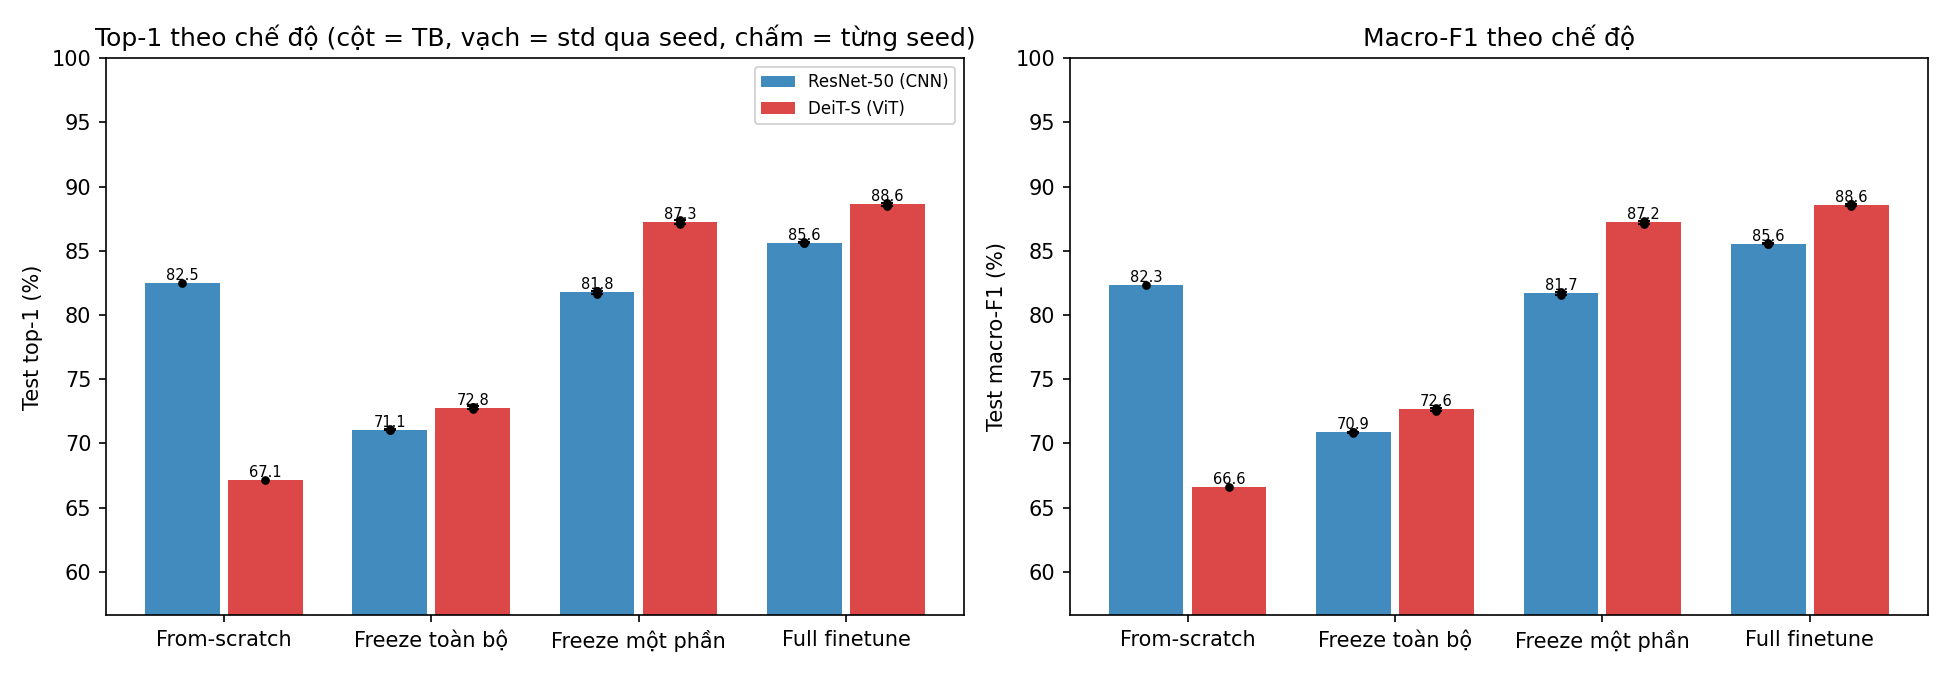
\includegraphics[width=\linewidth]{mode_compare.png}
\caption{Top-1 và macro-F1 trên test theo chế độ. Cột là trung bình, chấm đen là
từng seed. Độ lệch giữa các seed nhỏ đến mức các chấm gần như trùng nhau}
\label{fig:mode}
\end{figure}

Ba điểm nổi bật trong Bảng~\ref{tab:main}:
\begin{itemize}
\item Độ lệch chuẩn qua ba seed không vượt quá 0,14 điểm, trong khi khoảng cách giữa
hai mô hình ở cùng chế độ nhỏ nhất cũng là 1,73 điểm (freeze toàn bộ). Mọi so sánh
giữa các run pretrained vì thế đều lớn hơn nhiều so với nhiễu do seed.
\item Macro-F1 bám sát top-1 (chênh dưới 0,6 điểm) vì Food-101 cân bằng lớp. Dưới đây
nhóm dùng top-1 làm metric chính như protocol.
\item Thứ hạng của hai mô hình đảo chiều giữa from-scratch và ba chế độ có pretrain.
Đây là kết quả trung tâm của bài, được phân tích ở mục~\ref{sec:q1}.
\end{itemize}

\subsection{Đường cong huấn luyện}

\begin{figure}[H]
\centering
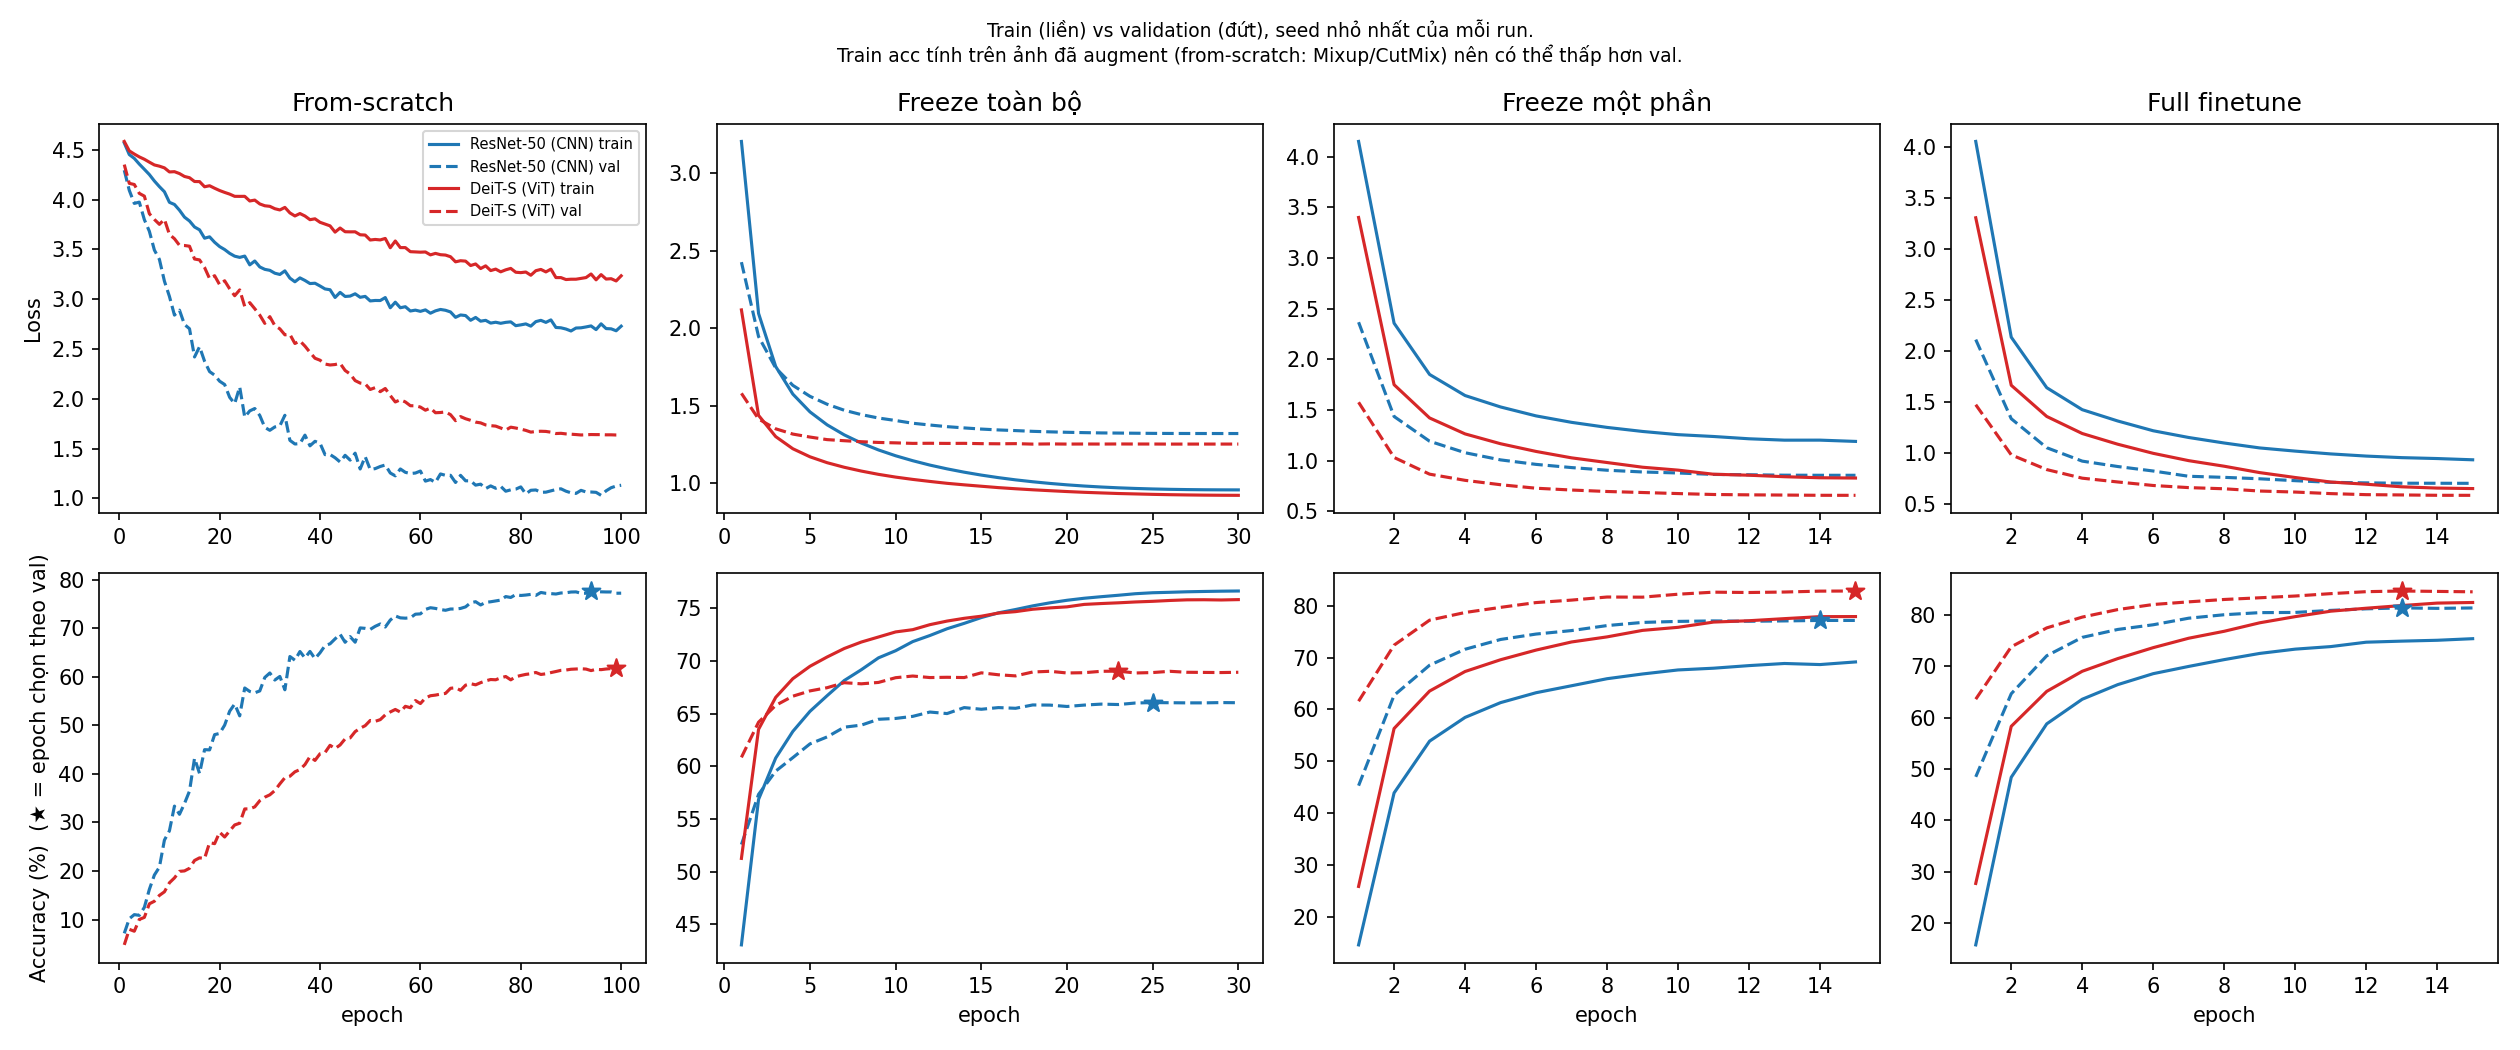
\includegraphics[width=\linewidth]{curves_by_mode.png}
\caption{Loss (hàng trên) và accuracy (hàng dưới) theo epoch, seed nhỏ nhất của mỗi
run. Nét liền là train, nét đứt là validation; ngôi sao đánh dấu epoch được chọn
theo validation}
\label{fig:curves}
\end{figure}

Hình~\ref{fig:curves} cho thấy mỗi chế độ hội tụ theo một kiểu khác nhau:
\begin{itemize}
\item \textbf{From-scratch:} validation của cả hai mô hình tăng gần như suốt 100
epoch và chỉ chững lại khi LR theo cosine về gần 0. Epoch tốt nhất là 94 (ResNet-50)
và 99 (DeiT-S), nên không có dấu hiệu overfit; giới hạn nằm ở lịch huấn luyện chứ
không nằm ở overfit. Sau khoảng 10 epoch đầu, đường validation của ResNet-50 luôn nằm trên DeiT-S.
Train accuracy không có ý nghĩa ở chế độ này vì nhãn đã bị Mixup/CutMix trộn, nên
hình chỉ vẽ train loss.
\item \textbf{Freeze toàn bộ:} train accuracy (khoảng 76\%) cao hơn validation
(66--69\%) gần 10 điểm, và validation đứng yên sau khoảng 15 epoch. Lớp tuyến tính đã
khai thác hết những gì feature ImageNet cố định có thể tách được. Khoảng cách
train--validation lớn một phần do chế độ này không có augmentation.
\item \textbf{Freeze một phần và full finetune:} validation cao hơn train trong suốt
quá trình. Nguyên nhân là train được đo trên ảnh đã qua RandAugment, RandomErasing và
drop path, còn validation đo trên ảnh sạch. Validation vẫn còn nhích lên ở các epoch
cuối, epoch tốt nhất thường là 13--15/15.
\end{itemize}

% =====================================================================
\section{Phân tích}
\label{sec:analysis}

\subsection{Câu hỏi 1: Pretrain giúp mỗi kiến trúc đến mức nào?}
\label{sec:q1}

\begin{figure}[H]
\centering
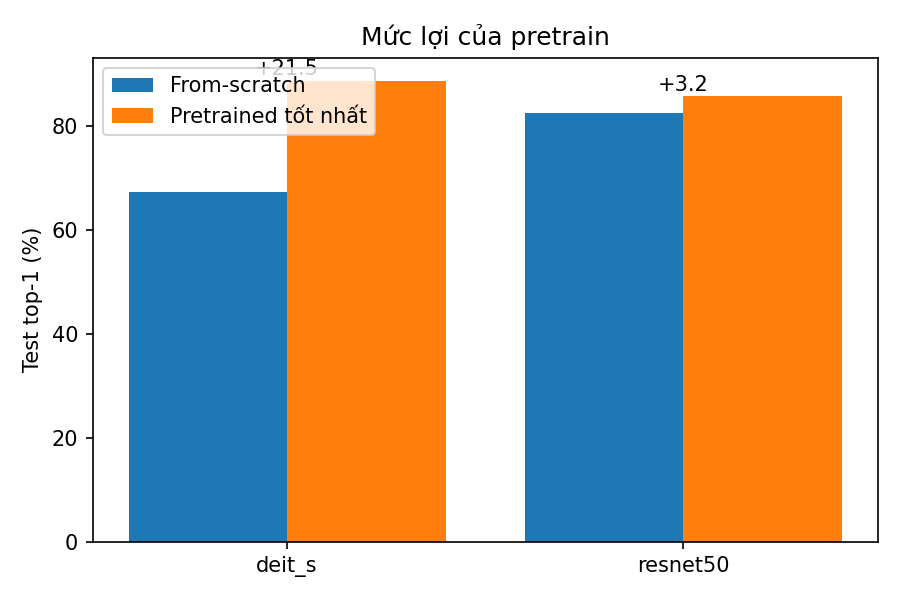
\includegraphics[width=0.7\linewidth]{pretrain_gap.png}
\caption{Top-1 của from-scratch so với run pretrained tốt nhất của mỗi mô hình}
\label{fig:gap}
\end{figure}

\begin{table}[H]
\centering
\caption{Khoảng cách pretrained -- from-scratch (top-1 trên test, \%)}
\label{tab:gap}
\begin{tabular}{lccc}
\toprule
Mô hình & From-scratch & Pretrained tốt nhất (full finetune) & Khoảng cách \\
\midrule
ResNet-50 & 82,48 & 85,65 & +3,16 \\
DeiT-S & 67,13 & 88,62 & +21,49 \\
\bottomrule
\end{tabular}
\end{table}

Kết quả khớp với kỳ vọng ban đầu, và chênh lệch giữa hai kiến trúc lớn hơn nhóm dự
đoán. Pretrain giúp DeiT-S thêm 21,5 điểm, gấp gần 7 lần mức 3,2 điểm của ResNet-50.

Với cùng 68 nghìn ảnh, cùng 100 epoch và cùng công thức augmentation, ResNet-50 train
từ đầu đạt 82,48\%, chỉ kém bản full finetune 3,2 điểm và thậm chí cao hơn bản freeze
một phần của chính nó (81,77\%). Convolution đã có sẵn tính cục bộ và chia sẻ trọng
số, nên mạng chỉ cần học \emph{nội dung} của các bộ lọc. DeiT-S thì phải học từ dữ
liệu cả việc ``điểm ảnh gần nhau thường liên quan với nhau''. Với lượng dữ liệu ít
hơn ImageNet khoảng 19 lần, DeiT-S chỉ đạt 67,13\%, kém ResNet-50 15,4 điểm. Kiểm định
McNemar ở mục~\ref{sec:agree} cho thấy ở chế độ from-scratch, số ảnh chỉ ResNet-50
đoán đúng gấp gần 6 lần số ảnh chỉ DeiT-S đoán đúng.

Khi có pretrain, thứ hạng đảo chiều: DeiT-S vượt ResNet-50 ở cả ba chế độ còn lại.
Một khi đã học được cấu trúc không gian từ ImageNet, attention toàn cục trở thành lợi
thế thay vì gánh nặng. DeiT-S nối được các vùng xa nhau trong ảnh (ví dụ nước sốt ở
một góc và miếng thịt ở giữa đĩa) ngay từ các block đầu, còn ResNet-50 chỉ có trường
nhìn rộng ở các stage cuối.

Có hai điều cần lưu ý khi diễn giải các con số này. Thứ nhất, from-scratch chỉ có một
seed. Tuy vậy, độ lệch giữa các seed của run pretrained không quá 0,14 điểm, rất nhỏ
so với khoảng cách 15 điểm, nên kết luận về hướng chênh lệch khó bị đảo. Thứ hai,
DeiT gốc được train 300 epoch trên 1,28 triệu ảnh [3]. Với 100 epoch, DeiT-S ở đây có
thể chưa đạt hết khả năng, vì validation vẫn còn tăng đến khi LR về 0. Kết luận chính
xác là: \emph{ở ngân sách huấn luyện và lượng dữ liệu này}, ViT thuần phụ thuộc vào
pretrain nhiều hơn CNN rất rõ.

\subsection{Câu hỏi 2: Mức freeze nào cân bằng accuracy và chi phí?}
\label{sec:q2}

\begin{figure}[H]
\centering
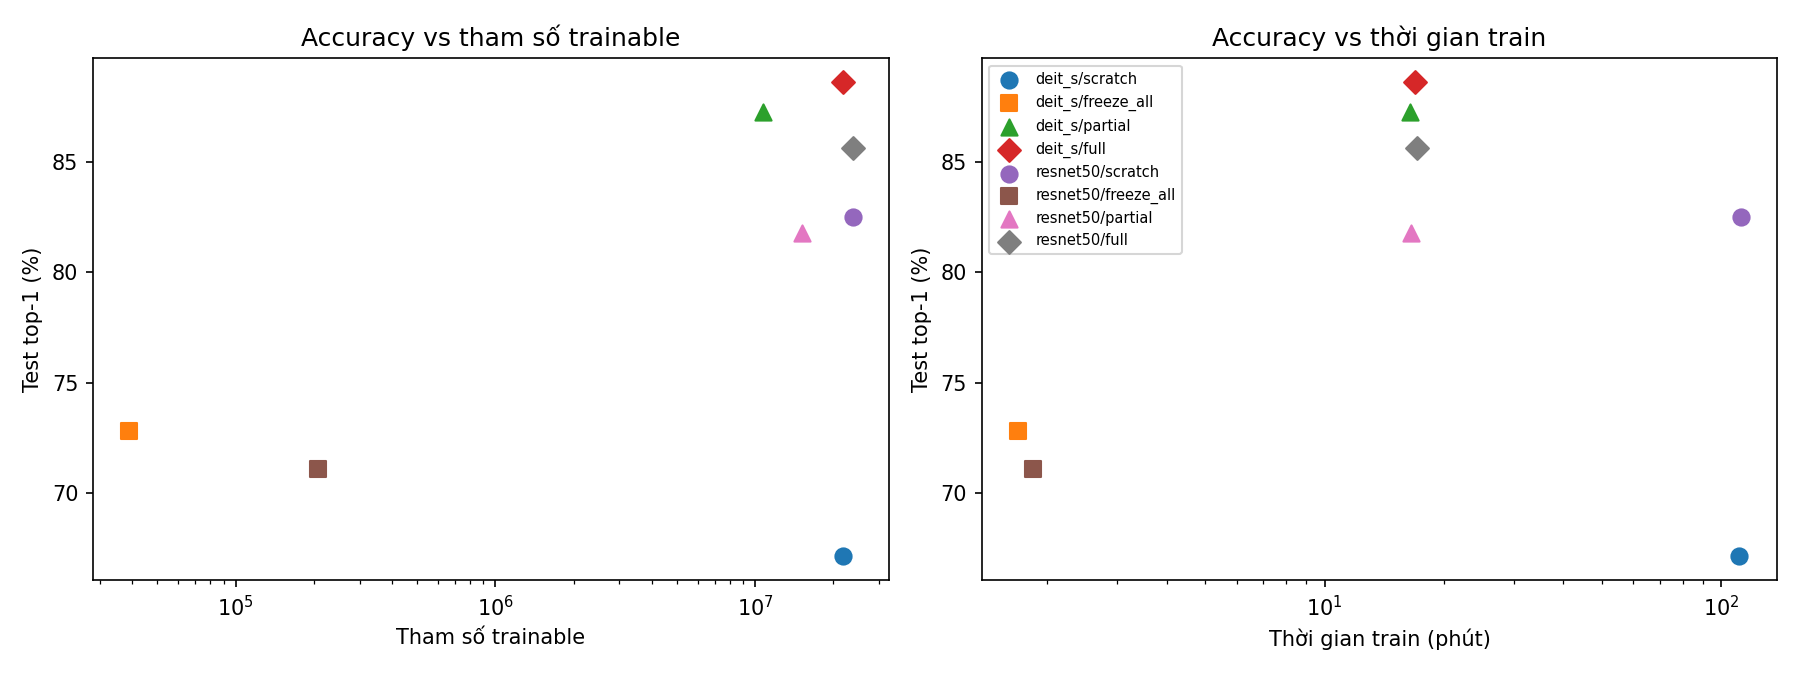
\includegraphics[width=\linewidth]{tradeoff.png}
\caption{Top-1 theo số tham số trainable (trái) và theo thời gian train (phải), trục
hoành logarit}
\label{fig:tradeoff}
\end{figure}

\begin{figure}[H]
\centering
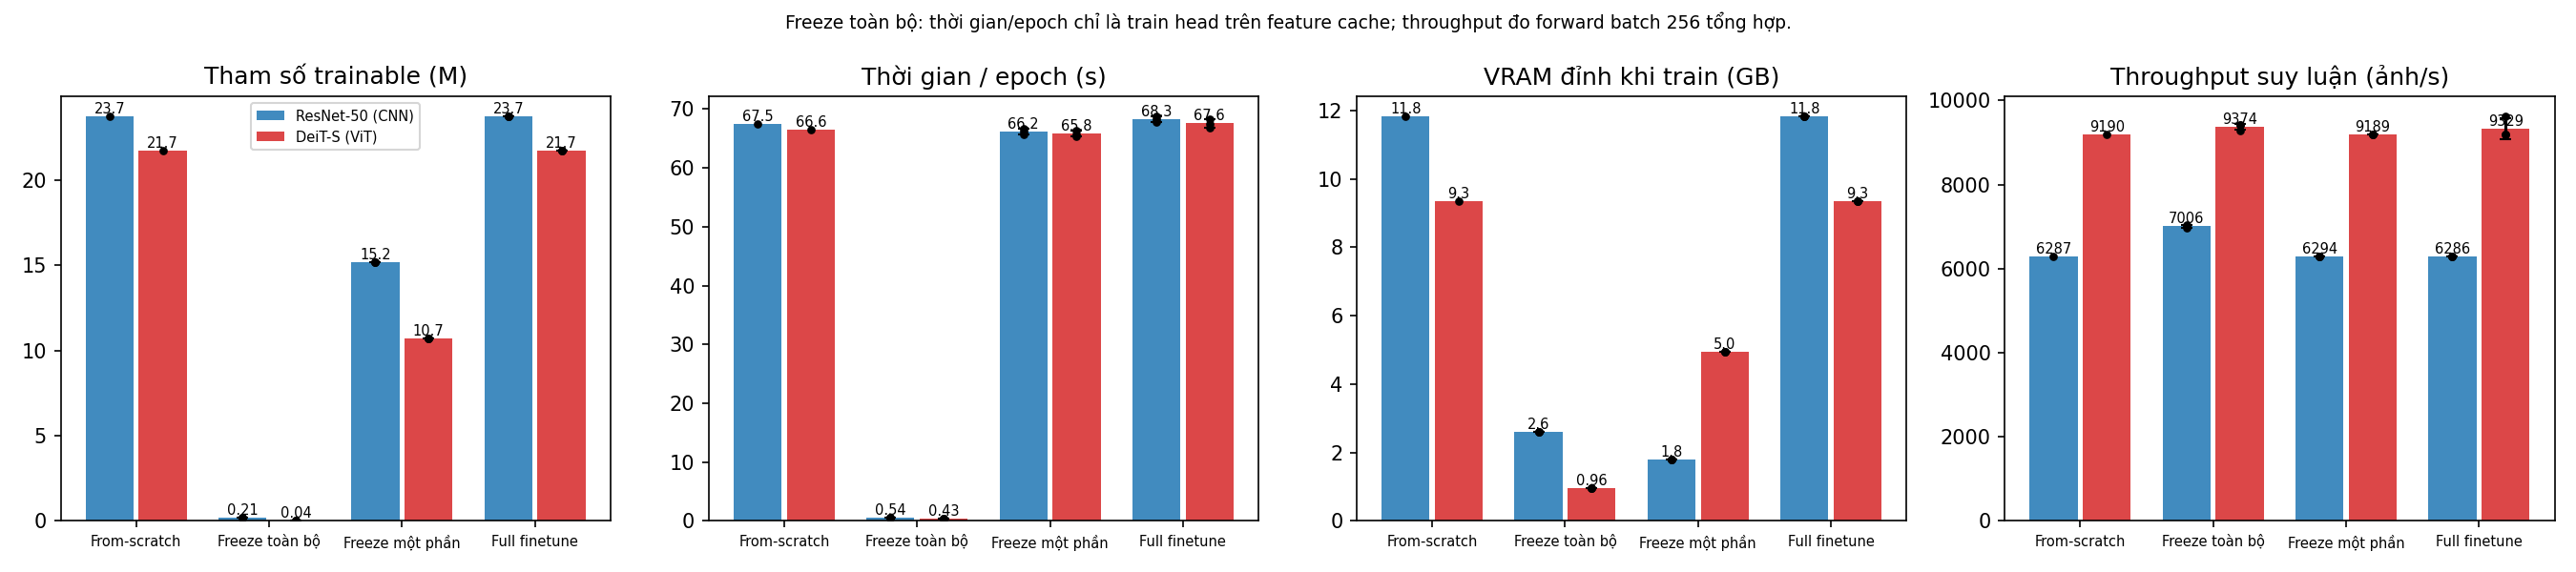
\includegraphics[width=\linewidth]{efficiency.png}
\caption{Chi phí theo chế độ: số tham số trainable, thời gian mỗi epoch, VRAM đỉnh
khi train, và throughput suy luận (forward batch 256, bf16, đầu vào tổng hợp)}
\label{fig:efficiency}
\end{figure}

\paragraph{Accuracy.} Bước nhảy lớn nhất nằm giữa freeze toàn bộ và freeze một phần:
+10,7 điểm với ResNet-50 và +14,5 điểm với DeiT-S. Feature ImageNet cố định chưa đủ
để tách các món ăn có chi tiết tinh tế; chỉ cần mở khóa nửa sau của mạng, mô hình đã
học lại được các đặc trưng cấp cao riêng cho món ăn. Từ freeze một phần lên full
finetune, DeiT-S chỉ được thêm 1,37 điểm, còn ResNet-50 được thêm 3,88 điểm. Với
ResNet-50, train riêng layer4 (64\% tham số) chưa đủ: các feature trung gian ở
layer1--3 cũng cần thích nghi với món ăn.

\paragraph{Thời gian.} Đây là phát hiện nhóm không lường trước khi viết protocol:
freeze một phần \emph{không} nhanh hơn full finetune. Cả from-scratch, freeze một phần
và full finetune đều mất 65--68 giây mỗi epoch, cho cả hai mô hình. Throughput forward
của GPU là khoảng 6.300 ảnh/giây (ResNet-50) và 9.200 ảnh/giây (DeiT-S), tức một lượt
forward qua 68 nghìn ảnh chỉ mất 7--11 giây. Như vậy thời gian mỗi epoch bị chặn bởi
khâu đọc và giải mã JPEG cùng augmentation trên CPU, không bị chặn bởi GPU. Bỏ bớt
backward cho nửa đầu mạng không làm epoch ngắn lại. Chỉ freeze toàn bộ, nhờ đọc ảnh
đúng một lần để trích feature, mới tiết kiệm thời gian thật sự (khoảng 1,8 phút so
với khoảng 17 phút).

\paragraph{Bộ nhớ.} Freeze một phần tiết kiệm VRAM rõ rệt, nhưng mức tiết kiệm khác
nhau giữa hai kiến trúc vì cách chúng lưu activation:
\begin{itemize}
\item ResNet-50 giảm từ 11,8 GB xuống 1,8 GB. Phần lớn activation cần lưu cho backward
nằm ở các stage đầu, nơi feature map lớn ($56\times56$, $28\times28$). layer4 chỉ chạy
trên $7\times7$ nên rất nhẹ.
\item DeiT-S chỉ giảm từ 9,3 GB xuống 5,0 GB. Mọi block của ViT xử lý cùng 197 token
với cùng chiều 384, nên sáu block sau tốn bộ nhớ đúng bằng sáu block đầu. Bộ nhớ
giảm gần đúng một nửa, tương ứng với nửa số block.
\end{itemize}

\paragraph{Kết luận cho câu 2.} Với bài toán này:
\begin{itemize}
\item Nếu không bị giới hạn bộ nhớ, full finetune là lựa chọn tốt nhất: cùng thời gian
với freeze một phần nhưng accuracy cao hơn.
\item Freeze một phần đáng dùng khi GPU nhỏ, đặc biệt với DeiT-S: giữ 98,5\% accuracy
của full finetune (87,25 so với 88,62) với một nửa số tham số trainable và gần một
nửa VRAM. Với ResNet-50, freeze một phần giảm VRAM nhiều nhất nhưng mất gần 4 điểm.
\item Freeze toàn bộ phù hợp để thử nhanh hoặc làm baseline. Mỗi run chưa đến 2 phút
và gần như không tốn VRAM, nhưng kém full finetune 14--16 điểm.
\end{itemize}

\subsection{CNN và ViT có sai trên cùng những ảnh?}
\label{sec:agree}

Hai mô hình được đánh giá trên cùng 25.250 ảnh test, nên ngoài so sánh hai con số
accuracy, có thể đếm từng ảnh: ảnh nào cả hai đúng, ảnh nào chỉ một mô hình đúng.
Kiểm định McNemar [6] dùng đúng hai ô ``chỉ một bên đúng'' để kiểm tra xem chênh lệch có
ý nghĩa thống kê hay không, chặt chẽ hơn việc so hai tỉ lệ độc lập.

\begin{figure}[H]
\centering
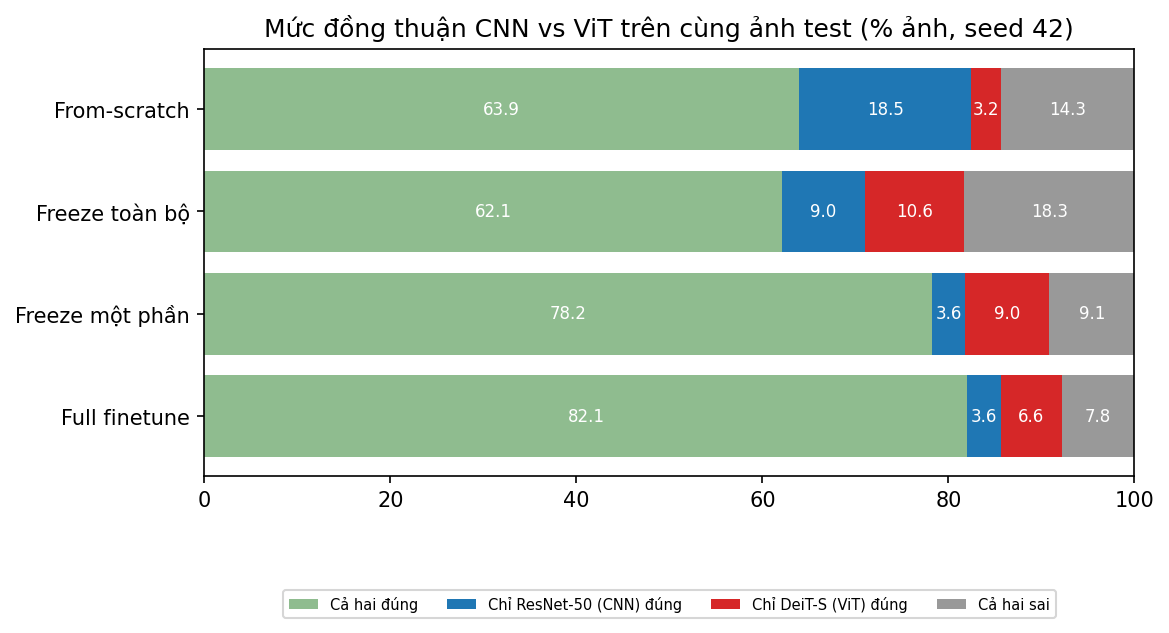
\includegraphics[width=0.85\linewidth]{agreement.png}
\caption{Tỉ lệ ảnh test theo bốn trường hợp đúng/sai của hai mô hình (seed 42)}
\label{fig:agree}
\end{figure}

\begin{table}[H]
\centering
\caption{Mức đồng thuận và kiểm định McNemar trên test (seed 42). ``Sai cùng nhãn'' là
tỉ lệ ảnh mà cả hai cùng đoán sai thành cùng một lớp}
\label{tab:mcnemar}
\resizebox{\linewidth}{!}{%
\begin{tabular}{lcccccrc}
\toprule
Chế độ & Cả hai đúng & Chỉ CNN & Chỉ ViT & Cả hai sai & Sai cùng nhãn & $\chi^2$ & $p$ \\
\midrule
From-scratch & 63,94 & 18,54 & 3,19 & 14,32 & 5,45 & 2736,1 & $<10^{-300}$ \\
Freeze toàn bộ & 62,07 & 9,01 & 10,62 & 18,30 & 7,06 & 33,1 & $8,8\cdot10^{-9}$ \\
Freeze một phần & 78,23 & 3,61 & 9,02 & 9,14 & 4,78 & 585,1 & $2,9\cdot10^{-129}$ \\
Full finetune & 82,06 & 3,60 & 6,55 & 7,79 & 4,36 & 216,0 & $6,8\cdot10^{-49}$ \\
\bottomrule
\end{tabular}}
\end{table}

Chênh lệch giữa hai mô hình có ý nghĩa thống kê ở cả bốn chế độ ($p < 10^{-8}$). Bảng
còn cho thấy thêm hai điều:
\begin{itemize}
\item Ngay ở full finetune, nơi DeiT-S tốt hơn rõ, vẫn có 3,6\% ảnh test chỉ
ResNet-50 đoán đúng. Hai mô hình mắc lỗi khác nhau một phần, nên nếu ghép chúng lại
(ensemble) thì trần lý thuyết, tức tỉ lệ ảnh có ít nhất một mô hình đúng, là 92,2\%.
\item Trong 7,79\% ảnh cả hai cùng sai, hơn một nửa (4,36\%) bị hai mô hình đoán sai
thành \emph{cùng một lớp}. Hai kiến trúc rất khác nhau mà vẫn đồng ý về câu trả lời
sai, nên nhiều khả năng các ảnh này mơ hồ thật sự: hai món giống nhau, hoặc ảnh có
nhiều món. Mục~\ref{sec:errors} kiểm tra điều này bằng mắt.
\end{itemize}

\begin{figure}[H]
\centering
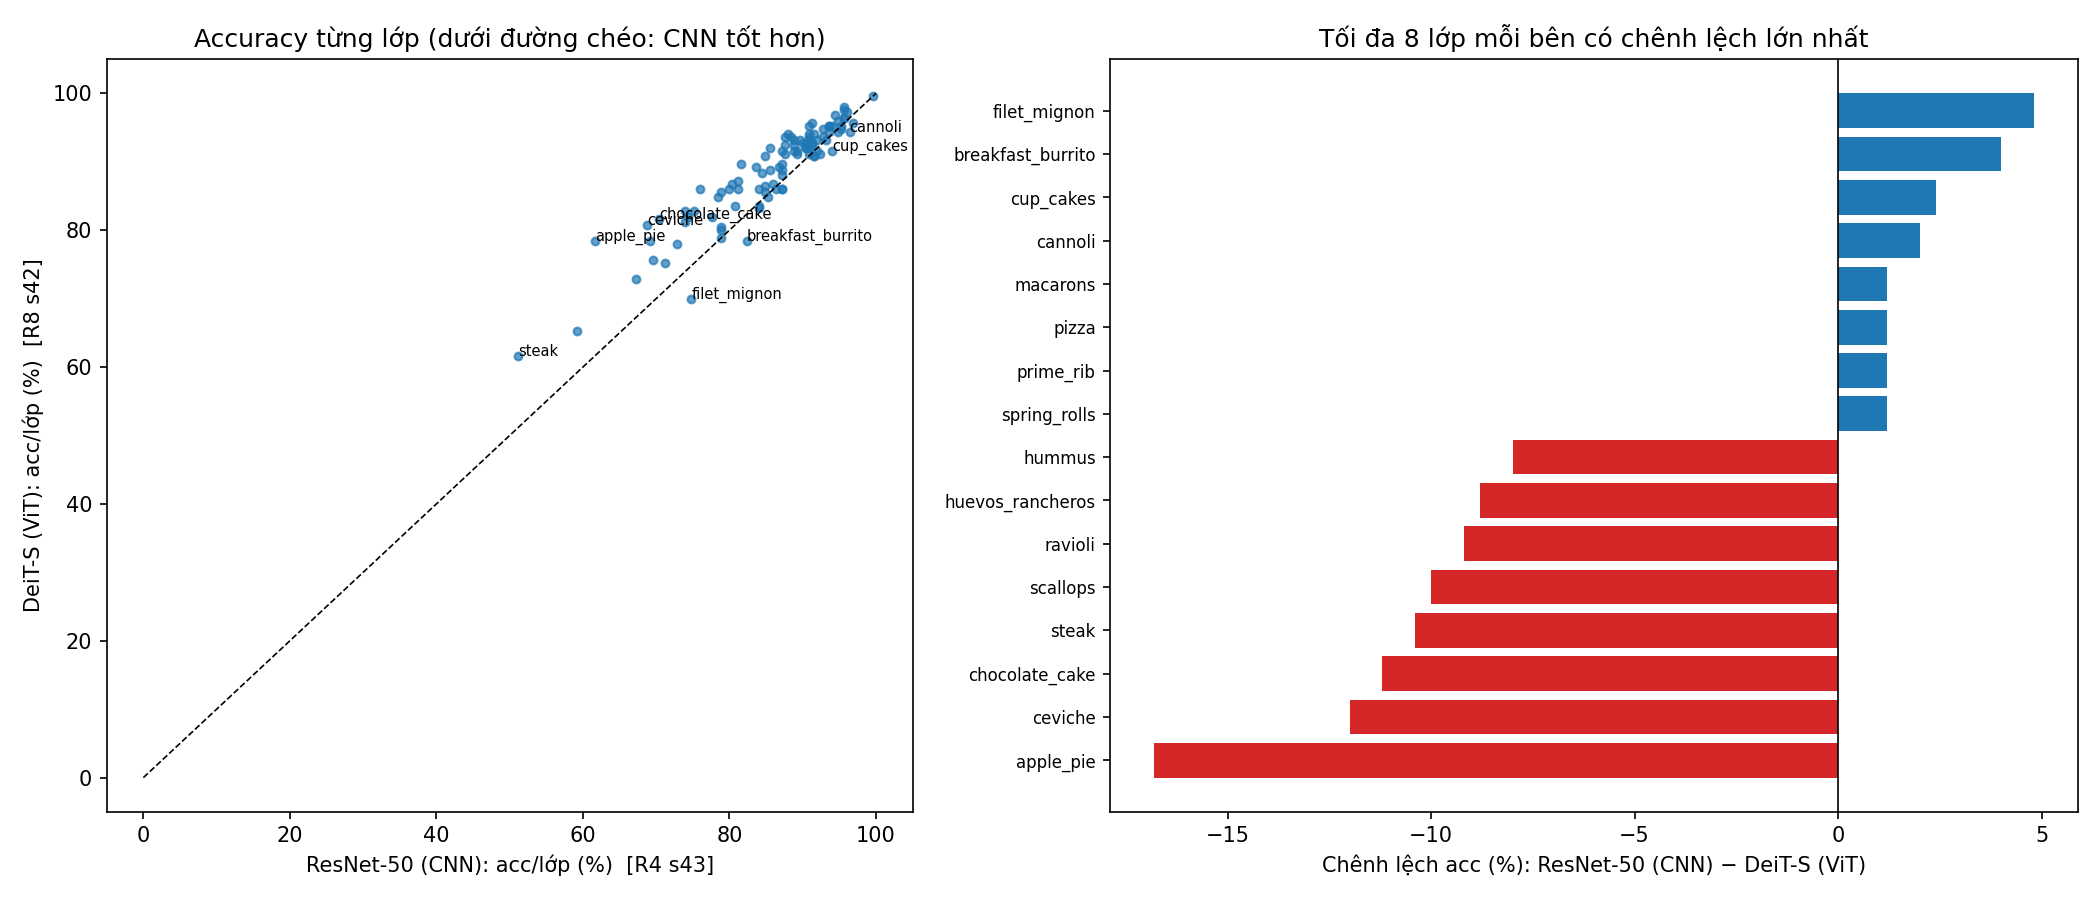
\includegraphics[width=\linewidth]{per_class.png}
\caption{Accuracy từng lớp của run full finetune tốt nhất theo validation (ResNet-50:
R4 seed 43, DeiT-S: R8 seed 42). Trái: mỗi chấm là một lớp, nằm trên đường chéo là
DeiT-S tốt hơn. Phải: các lớp có chênh lệch lớn nhất}
\label{fig:perclass}
\end{figure}

Theo từng lớp, DeiT-S tốt hơn ở 80/101 lớp, ResNet-50 tốt hơn ở 17 lớp, 4 lớp bằng
nhau. DeiT-S tiến bộ nhiều nhất ở apple pie (+16,8 điểm), ceviche, chocolate cake,
steak và scallops. Đây là các món mà hình dạng tổng thể và bối cảnh trên đĩa (lớp vỏ
bánh, cách bày, món ăn kèm) quan trọng hơn kết cấu bề mặt. ResNet-50 chỉ tốt hơn rõ ở
filet mignon (+4,8) và breakfast burrito (+4,0), và mức chênh nhỏ hơn hẳn.

\subsection{Phân tích lỗi}
\label{sec:errors}

\begin{figure}[H]
\centering
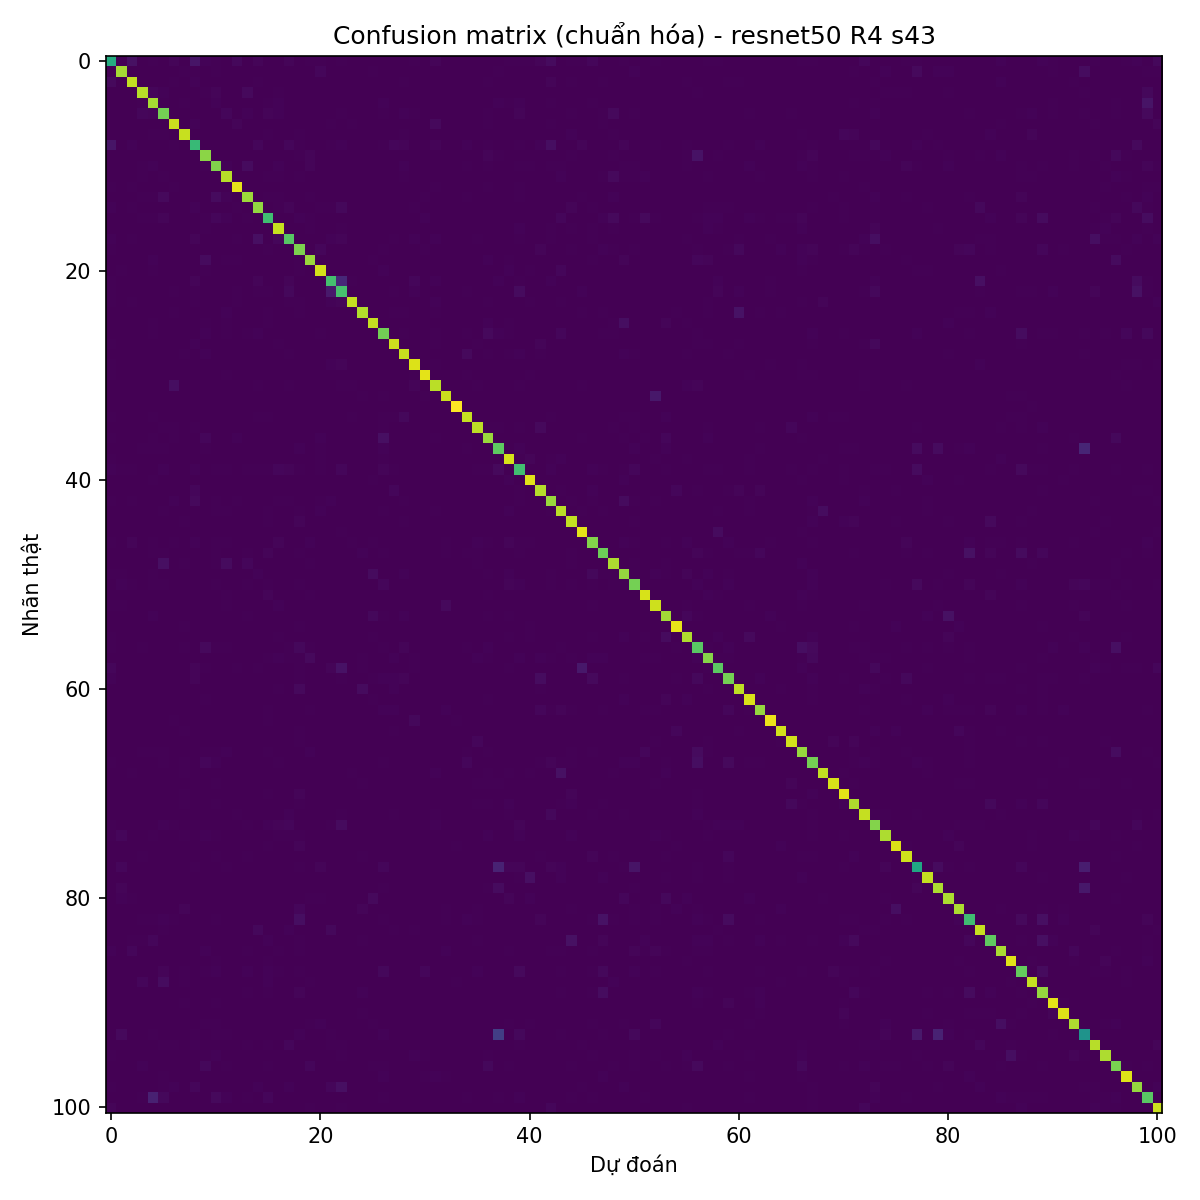
\includegraphics[width=0.49\linewidth]{confusion_resnet50.png}
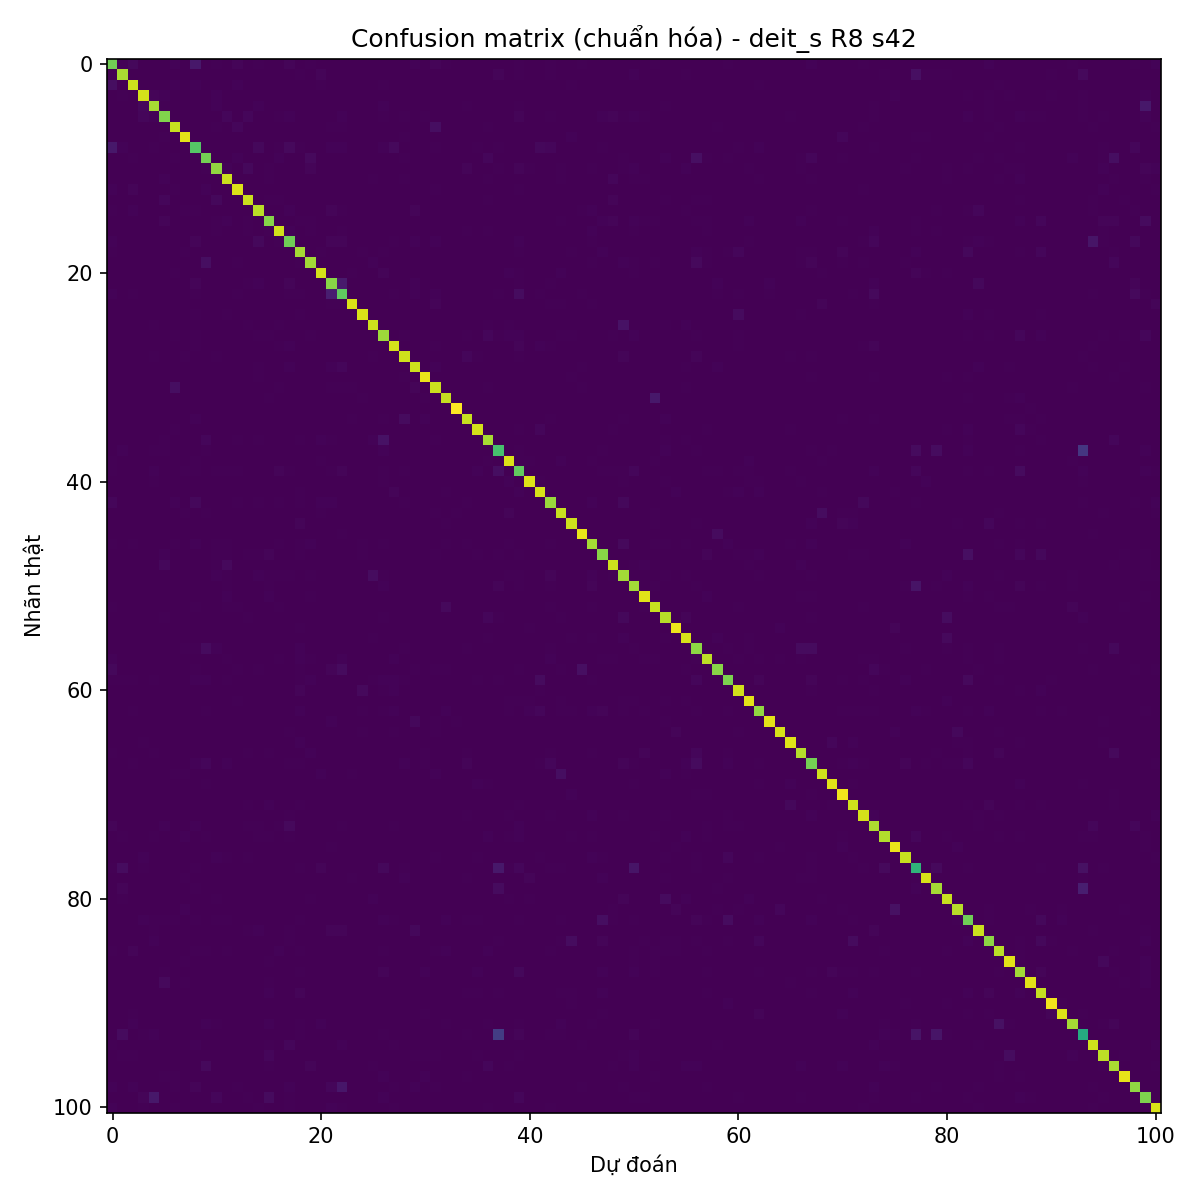
\includegraphics[width=0.49\linewidth]{confusion_deit_s.png}
\caption{Confusion matrix chuẩn hóa theo hàng của run tốt nhất mỗi mô hình (trái:
ResNet-50, phải: DeiT-S). Chỉ số lớp theo thứ tự bảng chữ cái trong
\texttt{splits/classes.json}}
\label{fig:confusion}
\end{figure}

Cả hai ma trận có đường chéo rõ, các ô nhầm rải rác và chỉ đậm ở một số cặp. Bảng
dưới liệt kê 10 cặp nhầm nhiều nhất.

\begin{table}[H]
\centering
\caption{10 cặp lớp bị nhầm nhiều nhất (số ảnh, trên 250 ảnh test mỗi lớp)}
\label{tab:pairs}
\small
\begin{tabular}{llr@{\hspace{2em}}llr}
\toprule
\multicolumn{3}{c}{ResNet-50 (R4 seed 43)} & \multicolumn{3}{c}{DeiT-S (R8 seed 42)} \\
Nhãn thật & Bị đoán thành & Ảnh & Nhãn thật & Bị đoán thành & Ảnh \\
\midrule
steak & filet mignon & 46 & steak & filet mignon & 44 \\
chocolate cake & chocolate mousse & 29 & filet mignon & steak & 39 \\
filet mignon & steak & 26 & chocolate mousse & chocolate cake & 21 \\
pork chop & filet mignon & 24 & prime rib & steak & 21 \\
steak & prime rib & 24 & chocolate cake & chocolate mousse & 18 \\
tuna tartare & beef tartare & 23 & beef tartare & tuna tartare & 16 \\
pork chop & steak & 20 & bread pudding & apple pie & 16 \\
steak & pork chop & 17 & dumplings & gyoza & 16 \\
chocolate mousse & chocolate cake & 17 & tuna tartare & beef tartare & 16 \\
prime rib & steak & 16 & apple pie & bread pudding & 16 \\
\bottomrule
\end{tabular}
\end{table}

Hai mô hình nhầm gần như cùng các cặp, và các cặp nhầm thường đi theo cả hai chiều
(steak $\leftrightarrow$ filet mignon, chocolate cake $\leftrightarrow$ chocolate mousse,
beef tartare $\leftrightarrow$ tuna tartare, apple pie $\leftrightarrow$ bread pudding).
Đây là dấu hiệu của các lớp thực sự chồng lấn về hình ảnh chứ không phải lỗi riêng
của một kiến trúc. Nhóm thịt nướng (steak, filet mignon, prime rib, pork chop) chiếm
7/10 cặp của ResNet-50. Steak là lớp khó nhất của cả hai mô hình (51\% với ResNet-50,
62\% với DeiT-S): nó vừa là tên chung cho cả nhóm, vừa trông giống ba lớp còn lại.

\begin{figure}[H]
\centering
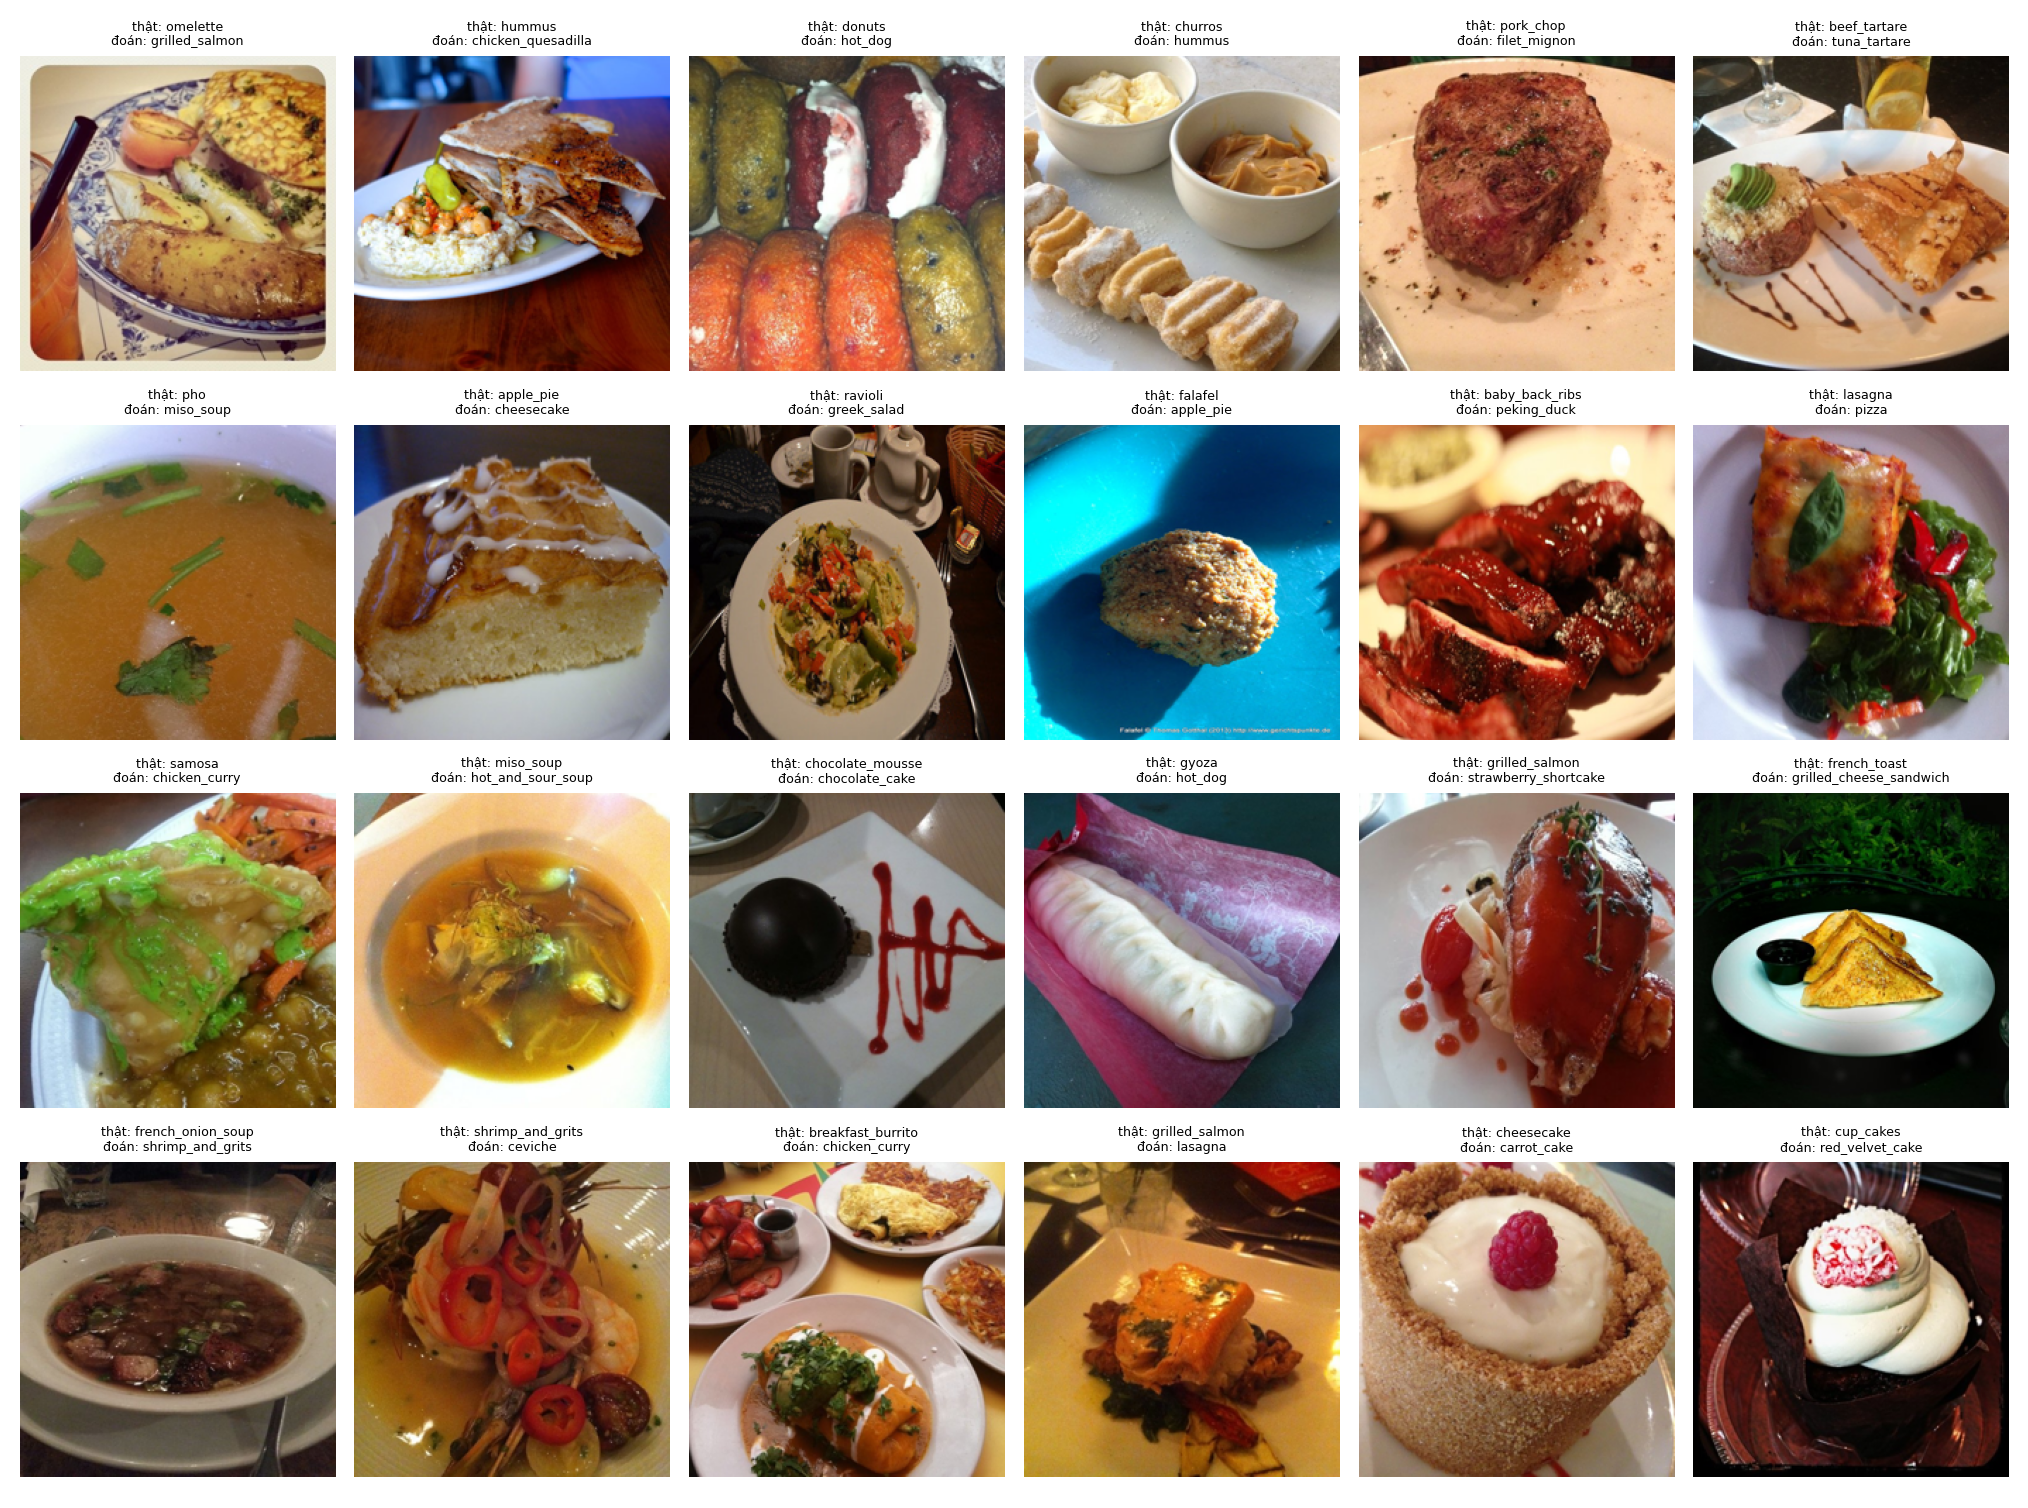
\includegraphics[width=\linewidth]{misclassified_resnet50.png}
\caption{24 ảnh test ResNet-50 đoán sai, chọn ngẫu nhiên (``thật'' là nhãn đúng,
``đoán'' là dự đoán top-1)}
\label{fig:mis-resnet}
\end{figure}

\begin{figure}[H]
\centering
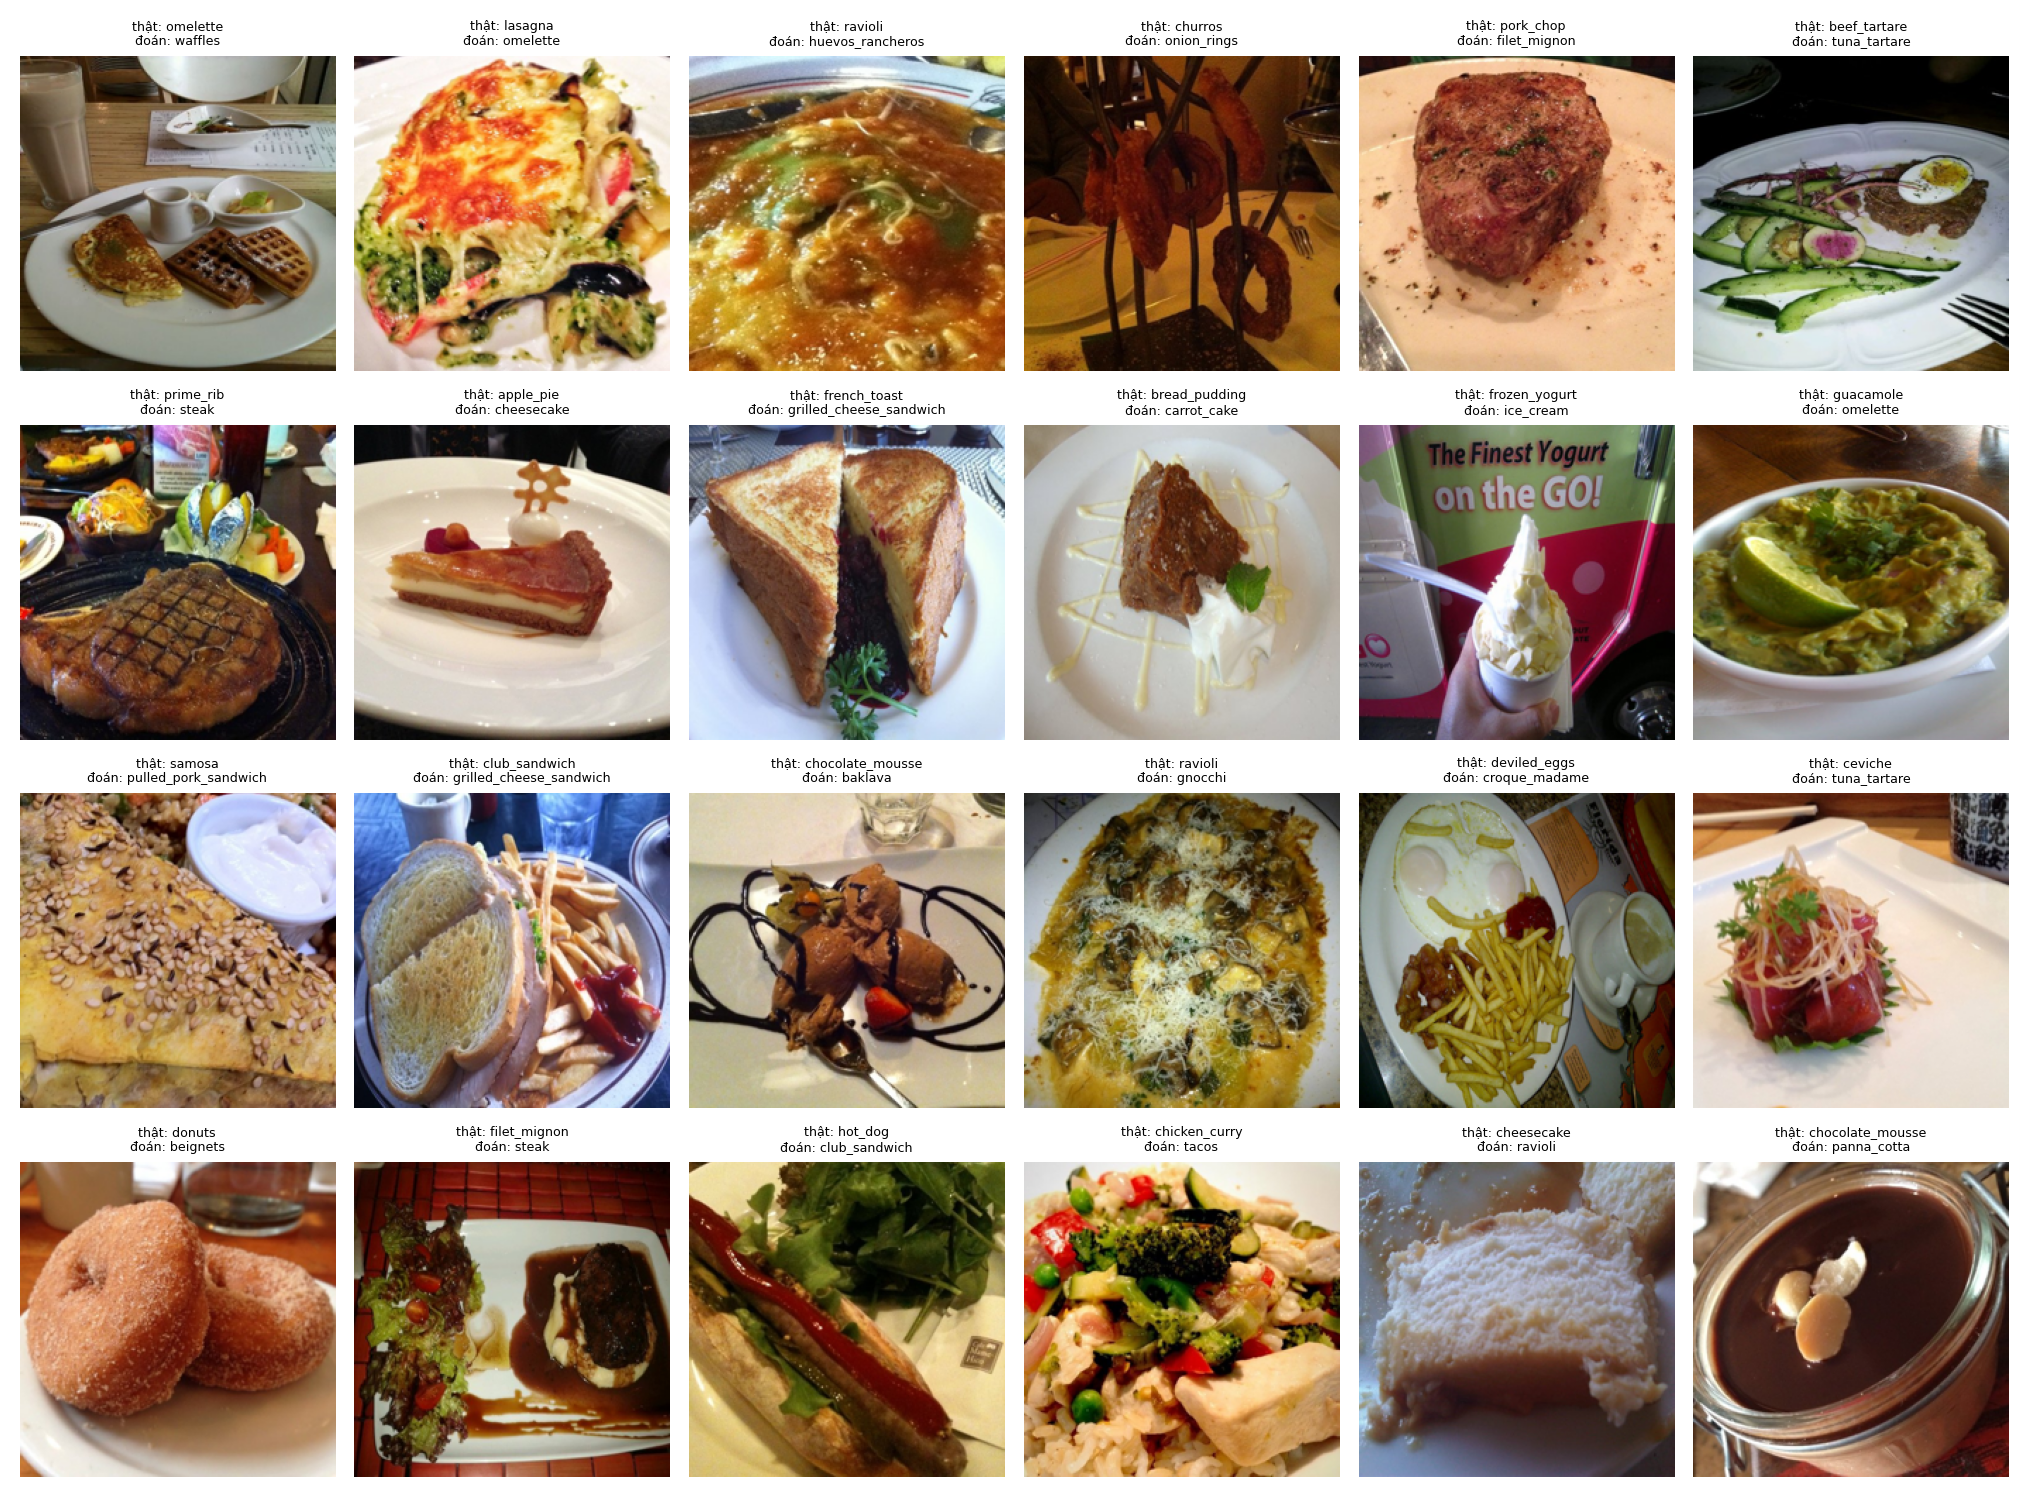
\includegraphics[width=\linewidth]{misclassified_deit_s.png}
\caption{24 ảnh test DeiT-S đoán sai, chọn ngẫu nhiên}
\label{fig:mis-deit}
\end{figure}

Nhóm xem lại 48 ảnh trong Hình~\ref{fig:mis-resnet} và~\ref{fig:mis-deit} và chia
nguyên nhân thành bốn nhóm, theo kế hoạch phân tích ở mục 8 của protocol:
\begin{enumerate}
\item \textbf{Hai món giống nhau thật sự.} Đây là nhóm lớn nhất: pork chop $\rightarrow$
filet mignon (xuất hiện ở cả hai lưới, cùng một ảnh), beef tartare $\rightarrow$ tuna
tartare, chocolate mousse $\rightarrow$ chocolate cake, prime rib $\rightarrow$ steak,
frozen yogurt $\rightarrow$ ice cream, french toast $\rightarrow$ grilled cheese sandwich
(cả hai mô hình). Nhiều ảnh trong nhóm này người không có kinh nghiệm ẩm thực cũng khó
phân biệt nếu chỉ nhìn ảnh.
\item \textbf{Ảnh có nhiều món.} Ảnh omelette có cả đĩa waffle bên cạnh, và DeiT-S trả
lời ``waffles''; ảnh breakfast burrito chụp cả một bàn ăn sáng; ảnh club sandwich có
đĩa khoai tây chiên chiếm nửa khung hình. Mô hình đoán đúng \emph{một} món trong ảnh,
chỉ không phải món được gán nhãn. Food-101 là bài toán một nhãn nên những ảnh này
không có câu trả lời ``đúng'' duy nhất.
\item \textbf{Cách trình bày bất thường.} Donuts cắt lát xếp hàng, gyoza gói trong
giấy trông như hot dog, falafel chụp trên nền xanh dương, churros đặt trên giá kim
loại. Các ảnh này lệch xa ``ảnh điển hình'' của lớp mà mô hình đã học.
\item \textbf{Ánh sáng và màu sắc kém.} Một số ảnh chụp trong nhà hàng tối hoặc bị ám
màu nặng (ravioli $\rightarrow$ huevos rancheros, lasagna $\rightarrow$ pizza), làm mất
chi tiết kết cấu.
\end{enumerate}

Nhóm không thấy ảnh nào rõ ràng bị gán nhãn sai trong 48 ảnh này, đúng với việc tập
test đã được tác giả kiểm tra thủ công. Nhiễu nhãn của Food-101 nằm ở tập train và
validation. Điều này cũng giải thích một hiện tượng nhất quán trong mọi run: test
top-1 luôn cao hơn validation top-1 khoảng 4--5 điểm (ví dụ R8 seed 42: validation
84,63\%, test 88,61\%). Validation được tách từ train nên chứa ảnh sai nhãn mà không
mô hình nào đoán ``đúng'' được.

% =====================================================================
\section{Giới hạn}
\label{sec:limits}

\begin{itemize}
\item \textbf{Chưa có cặp mở rộng.} Nhóm chưa chạy ConvNeXt-T và Swin-T (X1--X8), nên
chưa trả lời được câu 3: khoảng cách 21,5 điểm của DeiT-S đến từ attention nói chung
hay từ việc thiếu inductive bias cục bộ.
\item \textbf{From-scratch một seed, 100 epoch.} Hướng chênh lệch rất khó đảo vì nó
lớn gấp hơn 100 lần độ lệch seed của các run pretrained, nhưng con số tuyệt đối của
R5 có thể tăng nếu train lâu hơn.
\item \textbf{Lưới dò LR.} LR chọn cho ResNet-50 (3e-4) nằm ở biên trên của lưới. LR
tối ưu có thể còn cao hơn, và nếu vậy khoảng cách CNN--ViT ở các chế độ pretrained có
thể thu hẹp thêm. Protocol chỉ dò LR cho full finetune; chế độ freeze một phần dùng
lại giá trị đó mà không dò riêng.
\item \textbf{Freeze toàn bộ không có augmentation.} Do trích feature một lần, R2 và R6
không được augmentation như hai chế độ pretrained còn lại. Accuracy của chế độ này có
thể thấp hơn một chút so với bản có augmentation, đổi lại chi phí giảm gần 10 lần.
\item \textbf{Thời gian phụ thuộc pipeline dữ liệu.} Thời gian mỗi epoch phản ánh tốc
độ đọc ảnh và augmentation trên CPU của máy Colab, không phản ánh tốc độ tính toán của
mô hình. Throughput trong Hình~\ref{fig:efficiency} đo forward trên đầu vào tổng hợp
nên không gồm đọc ảnh.
\item \textbf{Hai loại A100.} Một số run chạy trên A100 80GB, số còn lại trên A100
40GB. Thời gian mỗi epoch đo được gần như bằng nhau, nhưng so sánh thời gian vẫn nên
đọc với sai số vài phần trăm.
\item \textbf{Pretrain khác recipe.} Hai bộ trọng số đều từ ImageNet-1k nhưng được huấn
luyện bằng các công thức khác nhau (\texttt{a1} của timm cho ResNet-50, công thức DeiT
cho DeiT-S), nên một phần chênh lệch ở các chế độ pretrained có thể đến từ chất lượng
pretrain chứ không chỉ từ kiến trúc.
\end{itemize}

% =====================================================================
\section{Kết luận}

\begin{enumerate}
\item \textbf{Pretrain quan trọng với ViT hơn nhiều so với CNN.} Train từ đầu trên 68
nghìn ảnh, ResNet-50 hơn DeiT-S 15,4 điểm. Có pretrain ImageNet-1k thì DeiT-S vượt lại
ở mọi chế độ. Pretrain giúp DeiT-S +21,5 điểm, giúp ResNet-50 +3,2 điểm.
\item \textbf{Full finetune DeiT-S cho kết quả tốt nhất}: 88,62 $\pm$ 0,10\% top-1,
hơn ResNet-50 khoảng 3 điểm ($p < 10^{-48}$, McNemar).
\item \textbf{Freeze một phần là điểm cân bằng tốt cho DeiT-S}: giữ 98,5\% accuracy với
một nửa tham số trainable và gần một nửa VRAM. Trên pipeline này, freeze một phần
không tiết kiệm thời gian; chỉ freeze toàn bộ tiết kiệm thời gian, nhưng mất 14--16
điểm.
\item \textbf{Dò learning rate làm thay đổi kết luận định lượng}: ResNet-50 cần LR
backbone lớn gấp ba DeiT-S. Dùng chung 1e-4 sẽ đánh giá thấp ResNet-50 khoảng 3,5
điểm.
\item \textbf{Lỗi còn lại chủ yếu do bản chất dữ liệu}: các cặp món giống nhau (nhóm
thịt nướng, hai món chocolate, hai món tartare) và ảnh có nhiều món. Hai kiến trúc
nhầm cùng các cặp, và hơn một nửa số ảnh cả hai cùng sai bị đoán thành cùng một lớp.
\end{enumerate}

% =====================================================================
\appendix
\section*{Phụ lục}
\addcontentsline{toc}{section}{Phụ lục}

\subsection*{P.1. Kết quả từng run}
\addcontentsline{toc}{subsection}{P.1. Kết quả từng run}

Bảng~\ref{tab:all} liệt kê mọi run đã chạy xong, kể cả bốn run dò LR không đưa vào
bảng chính (\texttt{R4\_s42}, \texttt{R4\_s42\_lr5e-05}, \texttt{R8\_s42\_lr0.0003},
\texttt{R8\_s42\_lr5e-05}). Run \texttt{R3\_s42} với LR 1e-4 bị dừng ở epoch 4 khi
bước dò LR chọn 3e-4 cho ResNet-50, và không được dùng. Các run smoke test
(\texttt{*\_smoke}) chỉ để kiểm tra code, không đưa vào báo cáo.

{\footnotesize
\begin{longtable}{llllcccccrc}
\caption{Kết quả từng run (\%). ``Epoch'' là epoch được chọn theo validation / tổng
số epoch; thời gian tính bằng phút}
\label{tab:all}\\
\toprule
Run & Seed & Thư mục & LR bb. & Epoch & Val & Test & Top-5 & F1 & Phút & GPU \\
\midrule
\endfirsthead
\toprule
Run & Seed & Thư mục & LR bb. & Epoch & Val & Test & Top-5 & F1 & Phút & GPU \\
\midrule
\endhead
R1 & 42 & \texttt{R1\_s42} & 5e-4 & 94/100 & 77,68 & 82,48 & 95,85 & 82,32 & 112,5 & 40GB \\
R2 & 42 & \texttt{R2\_s42} & --- & 25/30 & 66,05 & 71,08 & 91,57 & 70,87 & 1,8 & 80GB \\
R2 & 43 & \texttt{R2\_s43} & --- & 23/30 & 65,98 & 71,01 & 91,54 & 70,81 & 1,8 & 80GB \\
R2 & 44 & \texttt{R2\_s44} & --- & 29/30 & 66,06 & 71,10 & 91,58 & 70,89 & 1,8 & 80GB \\
R3 & 42 & \texttt{R3\_s42\_lr0.0003} & 3e-4 & 14/15 & 77,16 & 81,84 & 95,88 & 81,74 & 16,4 & 40GB \\
R3 & 43 & \texttt{R3\_s43\_lr0.0003} & 3e-4 & 12/15 & 77,27 & 81,64 & 95,89 & 81,55 & 16,7 & 40GB \\
R3 & 44 & \texttt{R3\_s44\_lr0.0003} & 3e-4 & 14/15 & 77,57 & 81,85 & 95,94 & 81,79 & 16,6 & 40GB \\
R4* & 42 & \texttt{R4\_s42\_lr5e-05} & 5e-5 & 14/15 & 75,12 & 79,68 & 95,10 & 79,49 & 17,2 & 40GB \\
R4* & 42 & \texttt{R4\_s42} & 1e-4 & 14/15 & 77,91 & 82,17 & 96,03 & 82,05 & 17,4 & 80GB \\
R4 & 42 & \texttt{R4\_s42\_lr0.0003} & 3e-4 & 13/15 & 81,35 & 85,66 & 97,18 & 85,61 & 17,0 & 40GB \\
R4 & 43 & \texttt{R4\_s43\_lr0.0003} & 3e-4 & 15/15 & 81,37 & 85,64 & 97,04 & 85,55 & 17,1 & 40GB \\
R4 & 44 & \texttt{R4\_s44\_lr0.0003} & 3e-4 & 13/15 & 81,07 & 85,64 & 97,12 & 85,54 & 17,2 & 40GB \\
R5 & 42 & \texttt{R5\_s42} & 5e-4 & 99/100 & 61,78 & 67,13 & 88,52 & 66,60 & 111,0 & 40GB \\
R6 & 42 & \texttt{R6\_s42} & --- & 23/30 & 69,03 & 72,69 & 92,31 & 72,53 & 1,7 & 80GB \\
R6 & 43 & \texttt{R6\_s43} & --- & 18/30 & 68,98 & 72,81 & 92,37 & 72,67 & 1,7 & 80GB \\
R6 & 44 & \texttt{R6\_s44} & --- & 19/30 & 69,08 & 72,86 & 92,38 & 72,73 & 1,7 & 80GB \\
R7 & 42 & \texttt{R7\_s42} & 1e-4 & 15/15 & 82,84 & 87,25 & 97,58 & 87,21 & 16,4 & 40GB \\
R7 & 43 & \texttt{R7\_s43} & 1e-4 & 14/15 & 82,52 & 87,40 & 97,59 & 87,34 & 16,6 & 40GB \\
R7 & 44 & \texttt{R7\_s44} & 1e-4 & 14/15 & 82,67 & 87,11 & 97,56 & 87,10 & 16,4 & 40GB \\
R8* & 42 & \texttt{R8\_s42\_lr5e-05} & 5e-5 & 15/15 & 83,51 & 88,02 & 97,86 & 87,98 & 16,6 & 40GB \\
R8 & 42 & \texttt{R8\_s42} & 1e-4 & 13/15 & 84,63 & 88,61 & 98,04 & 88,62 & 17,1 & 80GB \\
R8* & 42 & \texttt{R8\_s42\_lr0.0003} & 3e-4 & 14/15 & 84,58 & 88,84 & 97,97 & 88,81 & 16,6 & 40GB \\
R8 & 43 & \texttt{R8\_s43} & 1e-4 & 15/15 & 84,45 & 88,72 & 97,98 & 88,68 & 16,9 & 40GB \\
R8 & 44 & \texttt{R8\_s44} & 1e-4 & 14/15 & 84,46 & 88,52 & 97,96 & 88,52 & 16,7 & 40GB \\
\bottomrule
\multicolumn{11}{l}{* Run dò LR, không đưa vào bảng chính.}
\end{longtable}
}

Với DeiT-S, LR 3e-4 cho test cao hơn LR được chọn 0,23 điểm ở seed 42. Nhóm vẫn
giữ 1e-4 vì việc chọn LR chỉ dựa trên validation (84,63 so với 84,58), đúng như
protocol đã cam kết. Chênh lệch này cũng nằm trong khoảng dao động giữa các seed.

\subsection*{P.2. Tái lập}
\addcontentsline{toc}{subsection}{P.2. Tái lập}

\begin{itemize}
\item Notebook chạy trên Colab: \texttt{A1/notebooks/A1\_Colab.ipynb}. Chạy lần lượt
các cell; run đã xong được bỏ qua, run dở tiếp tục từ checkpoint.
\item Mã nguồn: \texttt{A1/src/}. \texttt{train.py} chứa vòng lặp huấn luyện,
\texttt{plan.py} thứ tự chạy và quy tắc chọn LR, \texttt{summarize.py} bảng và hình
của báo cáo này.
\item Mỗi run lưu \texttt{config.yaml}, \texttt{history.csv} (loss/accuracy theo epoch),
\texttt{metrics.json}, \texttt{confusion.npy} và \texttt{test\_preds.npz} trong
\texttt{A1/runs/<run>\_s<seed>/}. Checkpoint (\texttt{*.pt}) không đưa lên repository
vì dung lượng lớn.
\item Kết quả chọn LR: \texttt{A1/runs/lr\_selection.json}. Bảng tổng hợp:
\texttt{A1/summary.md}, \texttt{A1/summary.tex}, \texttt{A1/runs\_all.csv},
\texttt{A1/per\_class.csv}.
\end{itemize}

\subsection*{P.3. Khai báo hỗ trợ AI}
\addcontentsline{toc}{subsection}{P.3. Khai báo hỗ trợ AI}

Nhóm sử dụng AI để hỗ trợ hình thành ý tưởng: nên chọn mô hình nào để thể hiện rõ
tính chất và yêu cầu của bài tập, lựa chọn cách xây dựng pipeline, và tìm kiếm các
bộ dữ liệu phù hợp. Dựa trên đó, nhóm xác định kế hoạch chính, các bước cần có và
cần bổ sung. Về phần code, dựa vào kế hoạch đã xây dựng, nhóm dùng AI dựng sẵn một
khung template, rồi dựa vào đó để chỉnh sửa và thay đổi. Cuối cùng, nhóm dùng AI hỗ
trợ tổng hợp kết quả và viết báo cáo.

% =====================================================================
\section*{Tài liệu tham khảo}
\addcontentsline{toc}{section}{Tài liệu tham khảo}

\begin{enumerate}
\item[{[1]}] L. Bossard, M. Guillaumin, L. Van Gool. Food-101 -- Mining Discriminative
Components with Random Forests. ECCV 2014.
\url{https://data.vision.ee.ethz.ch/cvl/datasets_extra/food-101/}
\item[{[2]}] K. He, X. Zhang, S. Ren, J. Sun. Deep Residual Learning for Image
Recognition. CVPR 2016.
\item[{[3]}] H. Touvron, M. Cord, M. Douze, F. Massa, A. Sablayrolles, H. Jégou.
Training data-efficient image transformers \& distillation through attention. ICML
2021.
\item[{[4]}] A. Dosovitskiy và cộng sự. An Image is Worth 16x16 Words: Transformers for
Image Recognition at Scale. ICLR 2021.
\item[{[5]}] R. Wightman, H. Touvron, H. Jégou. ResNet strikes back: An improved training
procedure in timm. NeurIPS 2021 Workshop.
\item[{[6]}] Q. McNemar. Note on the sampling error of the difference between correlated
proportions or percentages. Psychometrika, 1947.
\end{enumerate}

\end{document}
